\documentclass{article}
\usepackage{listings}             % Include the listings-package
\usepackage[usenames,dvipsnames,svgnames,table]{xcolor}
\usepackage{graphicx}
\usepackage{hyperref}
\usepackage{amsmath}
\usepackage{amssymb}
\usepackage{amsthm}
\usepackage{csquotes}
\usepackage{changelog}
\usepackage{tabularx}
\usepackage{mathtools}
\usepackage{mdframed}
\usepackage{array}
\usepackage{float}
\usepackage{tikz}
\usepackage{soul}
\usepackage{makecell}
\usepackage{makeidx}
\usepackage{forest}

% Useful definitions for Math environments 
\newtheorem{theorem}{Theorem}[section]
\newtheorem{corollary}{Corollary}[theorem]
\newtheorem{lemma}[theorem]{Lemma}
\theoremstyle{definition}
\newtheorem{definition}{Definition}[section]
\newenvironment{remark}[1][Remark]{\begin{trivlist}
\item[\hskip \labelsep {\bfseries #1}]}{\end{trivlist}}

\newenvironment{dummy}{}{}

\definecolor{mygreen}{rgb}{0,0.6,0}
\definecolor{mygray}{rgb}{0.5,0.5,0.5}
\definecolor{mymauve}{rgb}{0.58,0,0.82}

\newcommand{\ChatDiamondVersion}{0.1.0-alpha}
\newcommand{\FileColor}[1]{{\color{Purple} #1}}
\newcommand{\FolderColor}[1]{{\color{mygray} #1}}

\lstdefinelanguage{cmake} {morekeywords={one,two,three,four,five,six,seven,eight,
nine,ten,eleven,twelve,o,clock,rock,around,the,tonight}, sensitive=false,
morecomment=[l]{//},
morecomment=[s]{/*}{*/},
morestring=[b]", }

% Container for tabularx
\floatstyle{plain}
\newfloat{tabcontainer}{thp}{lop}
\floatname{tabcontainer}{Table}

% Container for tikz flow-charts
\floatstyle{plain}
\newfloat{fccontainer}{thp}{lop}
\floatname{fccontainer}{FlowChart}

% For visual representation of Flow-Charts
\usetikzlibrary{shapes.geometric, arrows}
\tikzstyle{startstop} = [rectangle, rounded corners, minimum width=3cm, minimum height=1cm,text centered, draw=black, fill=red!30]
\tikzstyle{process} = [rectangle, minimum width=3cm, minimum height=1cm, text centered, draw=black, fill=orange!30]
\tikzstyle{arrow} = [thick,->,>=stealth]
    
\title{Chat Diamond}
\author{The\_Cowboy}
\pagestyle{headings}

\begin{document}

\maketitle
\tableofcontents

\lstset{language=Java}          % Set your language (you can change the language for each code-block optionally)

\bigskip

\textcolor{pink}{BIG FAT NOTE: Chat Diamond is in very early stages of development.  Please embrace yourselves for unexpected features and bugs here and there punctuated by tons of client logs.  If possible please raise an issue at \href{https://github.com/ravimohan1991/ChatDiamond/issues}{GitHub}!}

\section{Introduction}

\lstset{ %
  backgroundcolor=\color{white},   % choose the background color; you must add \usepackage{color} or    %\usepackage{xcolor}
  basicstyle=\footnotesize,        % the size of the fonts that are used for the code
  breakatwhitespace=false,         % sets if automatic breaks should only happen at whitespace
  breaklines=true,                 % sets automatic line breaking
  captionpos=b,                    % sets the caption-position to bottom
  commentstyle=\color{mygreen},    % comment style
  deletekeywords={...},            % if you want to delete keywords from the given language
  escapeinside={\%*}{*)},          % if you want to add LaTeX within your code
  extendedchars=true,              % lets you use non-ASCII characters; for 8-bits encodings only, %does not work with UTF-8
  frame=single,                    % adds a frame around the code
  keepspaces=true,                 % keeps spaces in text, useful for keeping indentation of code %(possibly needs columns=flexible)
  keywordstyle=\color{blue},       % keyword style
  language=Java,                 % the language of the code
  morekeywords={*,...},            % if you want to add more keywords to the set
  numbers=left,                    % where to put the line-numbers; possible values are (none, left, %right)
  numbersep=5pt,                   % how far the line-numbers are from the code
  numberstyle=\tiny\color{mygray}, % the style that is used for the line-numbers
  rulecolor=\color{black},         % if not set, the frame-color may be changed on line-breaks within %not-black text (e.g. comments (green here))
  showspaces=false,                % show spaces everywhere adding particular underscores; it %overrides 'showstringspaces'
  showstringspaces=false,          % underline spaces within strings only
  showtabs=false,                  % show tabs within strings adding particular underscores
  stepnumber=2,                    % the step between two line-numbers. If it's 1, each line will be %numbered
  stringstyle=\color{mymauve},     % string literal style
  tabsize=2,                       % sets default tabsize to 2 spaces
  title=\lstname                   % show the filename of files included with \lstinputlisting; also %try caption instead of title
} %optionally)

Chat Diamond (version \ChatDiamondVersion) is a purely client-side mod for Unreal Tournament G.O.T.Y (UT99) which replaces the default UT console with a more appropriate one.  This functionality allows the achievement of the following
\begin{itemize}
\item Gathering of raw messages delivered to the console and relevant categorization, along with chat message separation, of them.
\item Introduction of appropriate web-query for translation to local or demand of the language.
\end{itemize}

\begin{figure}
\centering
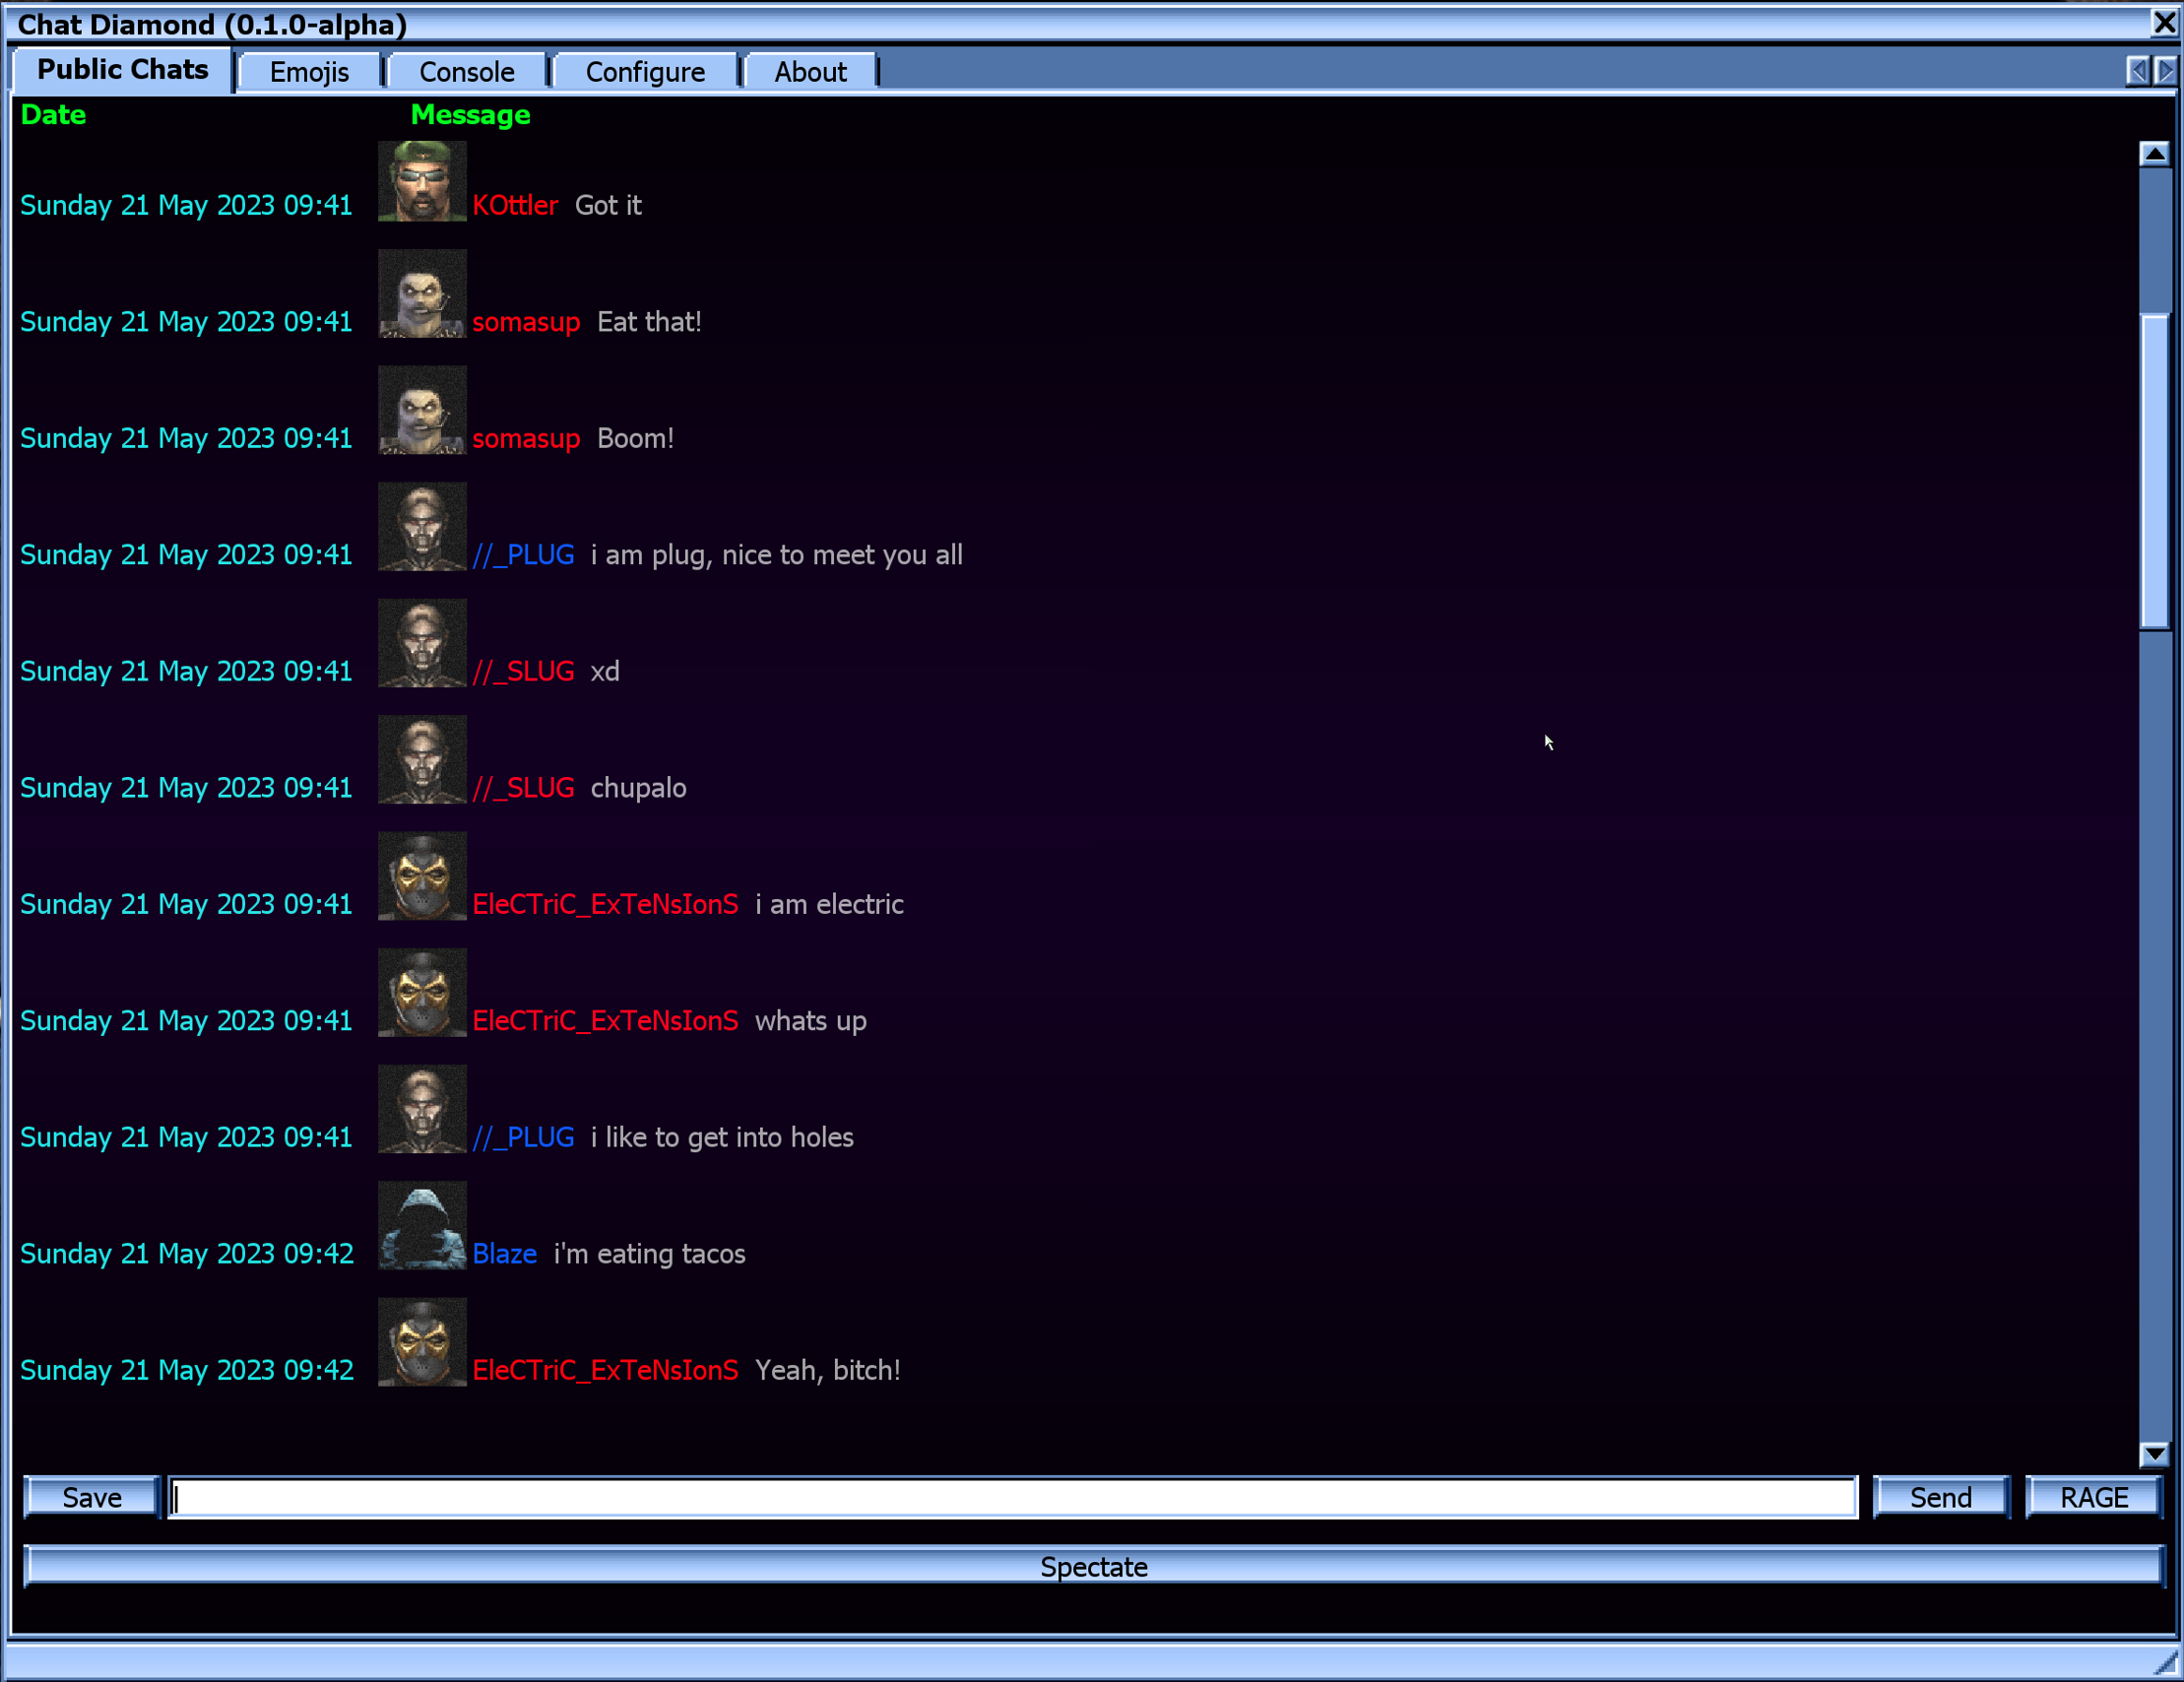
\includegraphics[width=0.4\textwidth]{img}
\caption{Chat Diamond \ChatDiamondVersion~Chat.}
\label{fig:chatdiamond}
\end{figure}

\subsection{Chat Window}
Figure \ref{fig:chatdiamond} shows the current form of the chat window. The following features are supported
\begin{itemize}
\item Display of sender's avatar face.
\item Static emojis and animated emotes.
\item Display of Date and Time (long format for now).
\item Display of the Server name for reference purposes.
\item Ability to copy text and IP address (both game and web server) from chat messages.
\begin{itemize}
\item IPs of the format xxx.xxx.xxx.xxx are considered web server IPs.
\item IPs of the format xxx.xxx.xxx.xxx:xxxx are considered game server IPs.
\end{itemize}
\item Ability to display hyperlinks with clickable feature for relevant navigation and mouse cursor distinction.
\begin{itemize}
\item On clicking web or game server IP, the player can reach the relevant website (http:// only) or UT99 game server.
\item On clicking http://something.com or https://something.com, the player can reach the desired site, if valid URL is posted.
\end{itemize}
\end{itemize}

\subsection{Emoji Window}

\begin{figure}
\centering
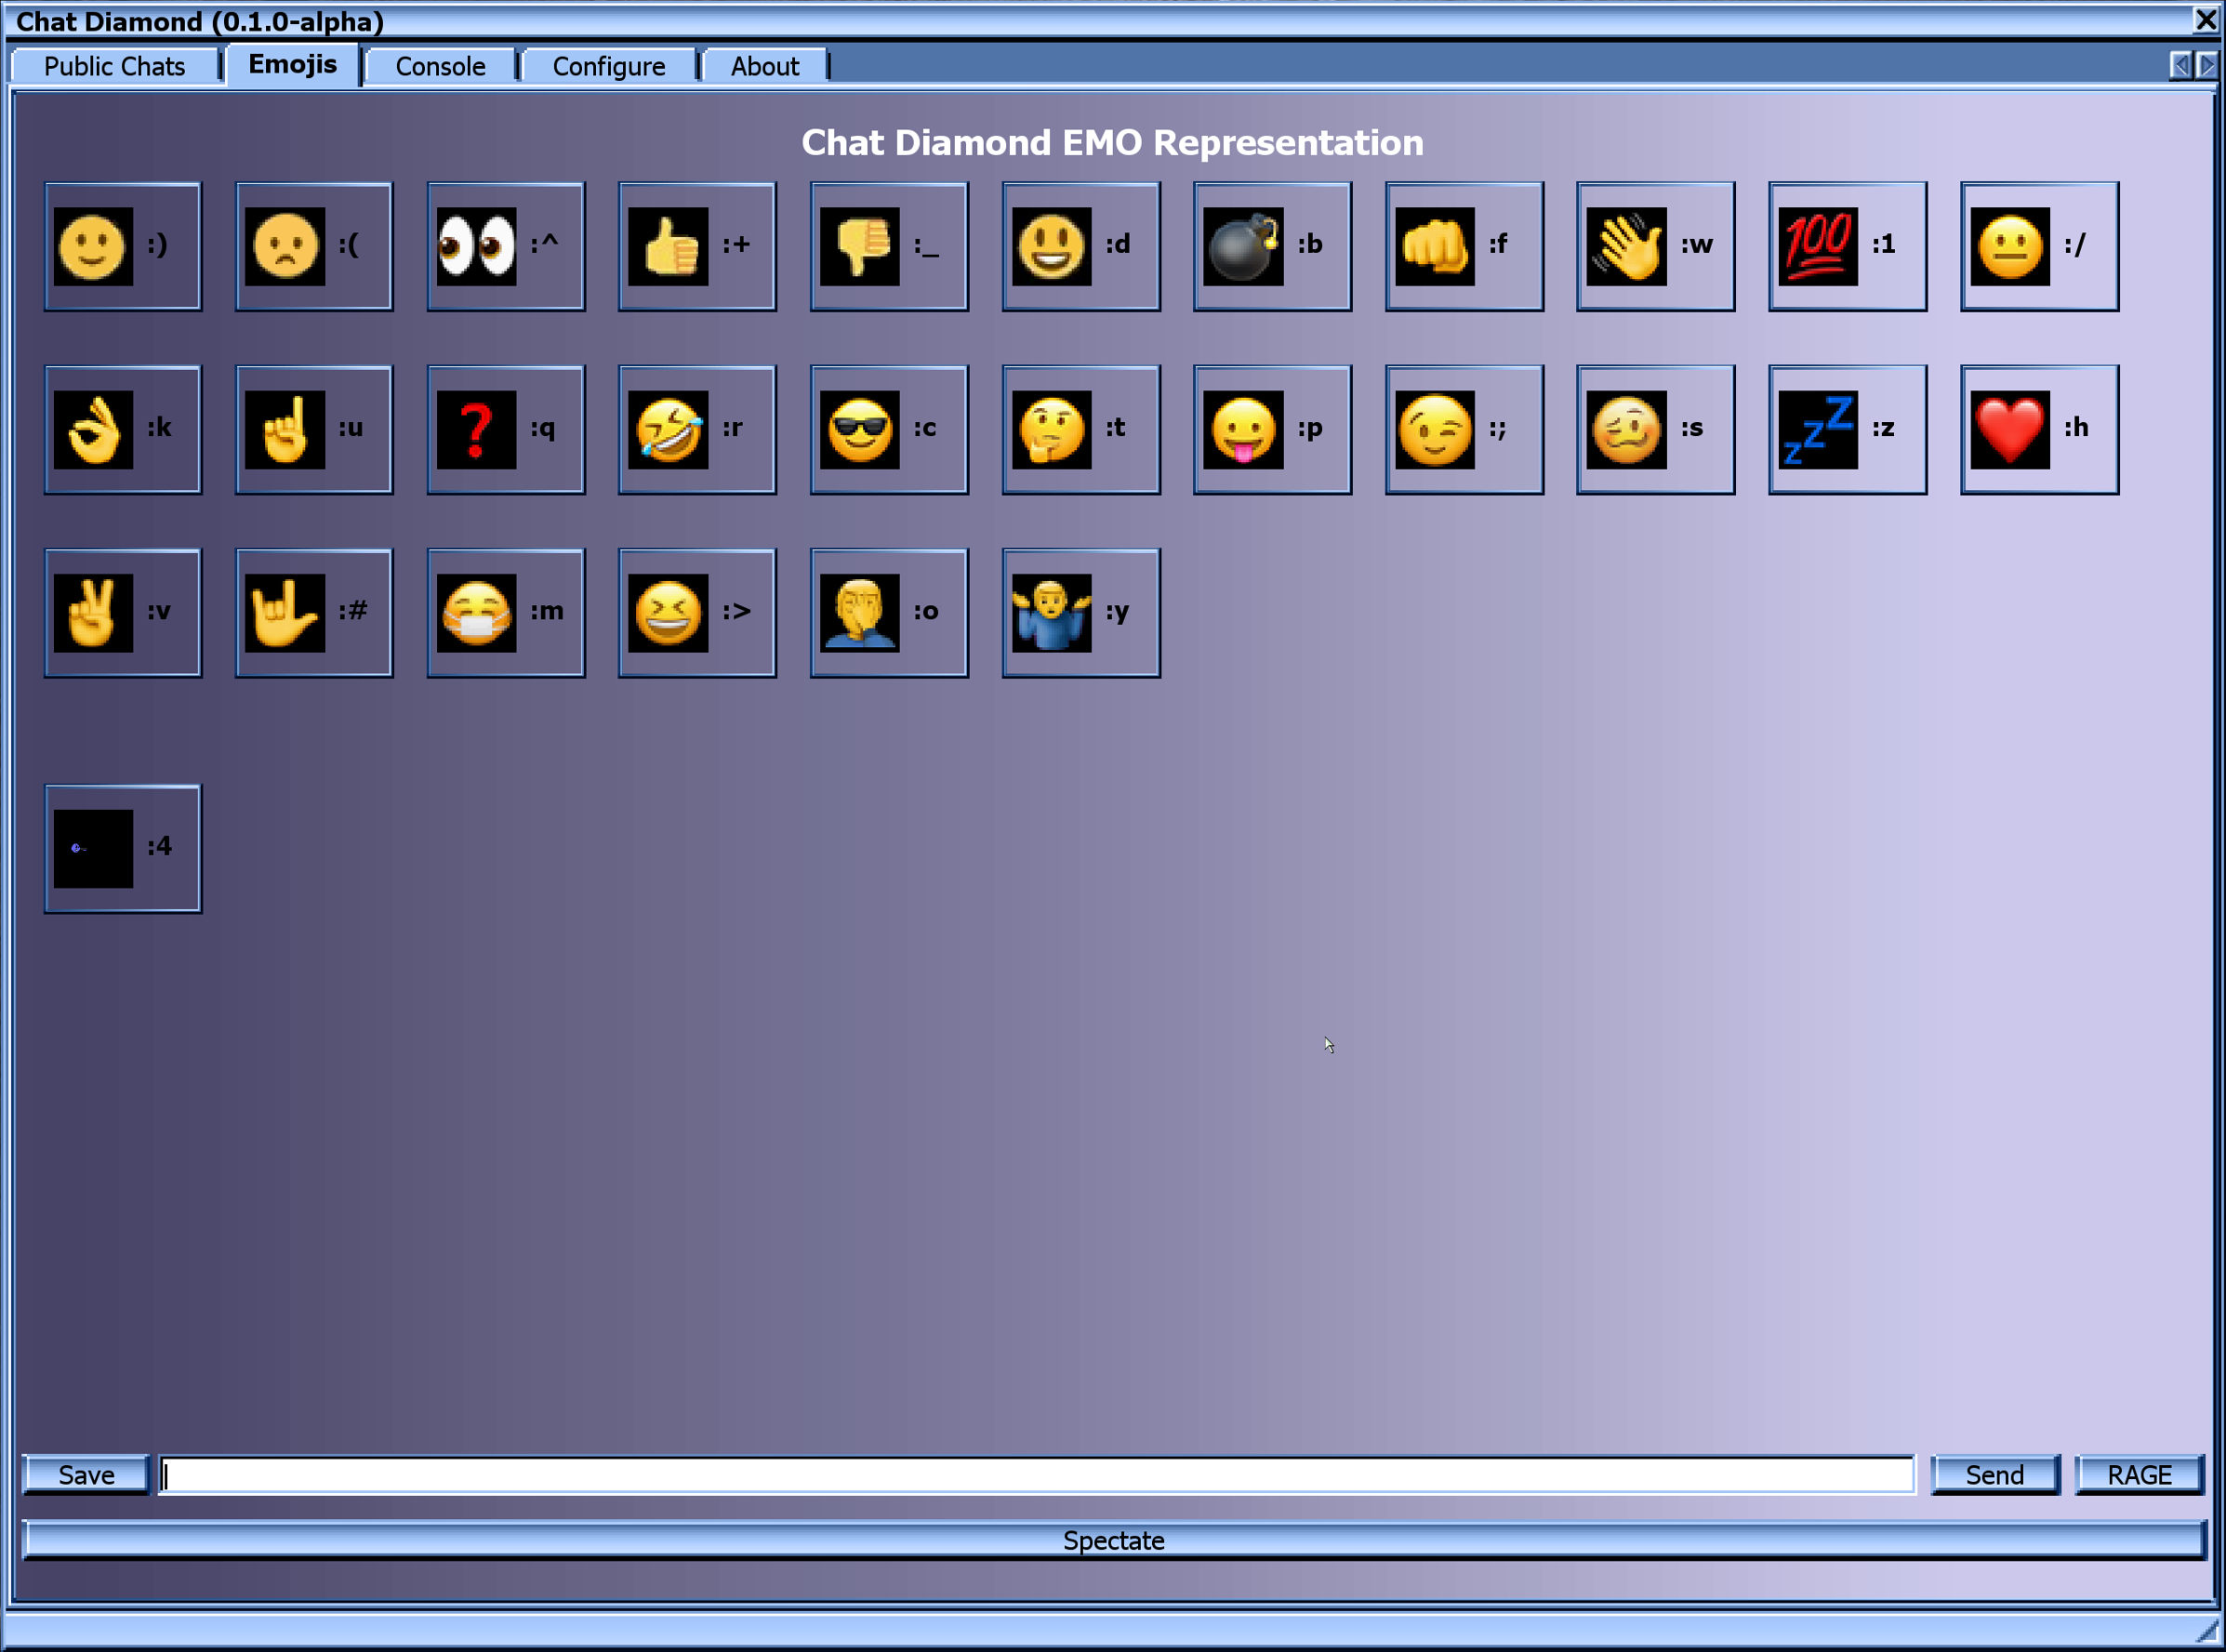
\includegraphics[width=0.4\textwidth]{img_emos}
\caption{Chat Diamond \ChatDiamondVersion~Emojis.}
\label{fig:chatdiamond_emos}
\end{figure}

In order to display complete list of supported emojis (and emotes), collectively called \emph{Emos}, the Emoji window \ref{fig:chatdiamond_emos} (which was texture based for UT Chat) has been 
written almost completely in unreal script (save the textures).  This allows the support for the following 
\begin{itemize}
\item A curation of selection page for framed Emos.
\item An interactive way of display, which depresses the frame being hovered with a sound and generates a distinct clicking
experience.
\item Emoji and Chat window text areas are synced, meaning, whatever you write or select in one window, which gets registered
in the text area, is copied over to the next one.
\item My personal favorite, the scrolling capability.
\end{itemize}


\subsection{Console Window}

\begin{figure}
\centering
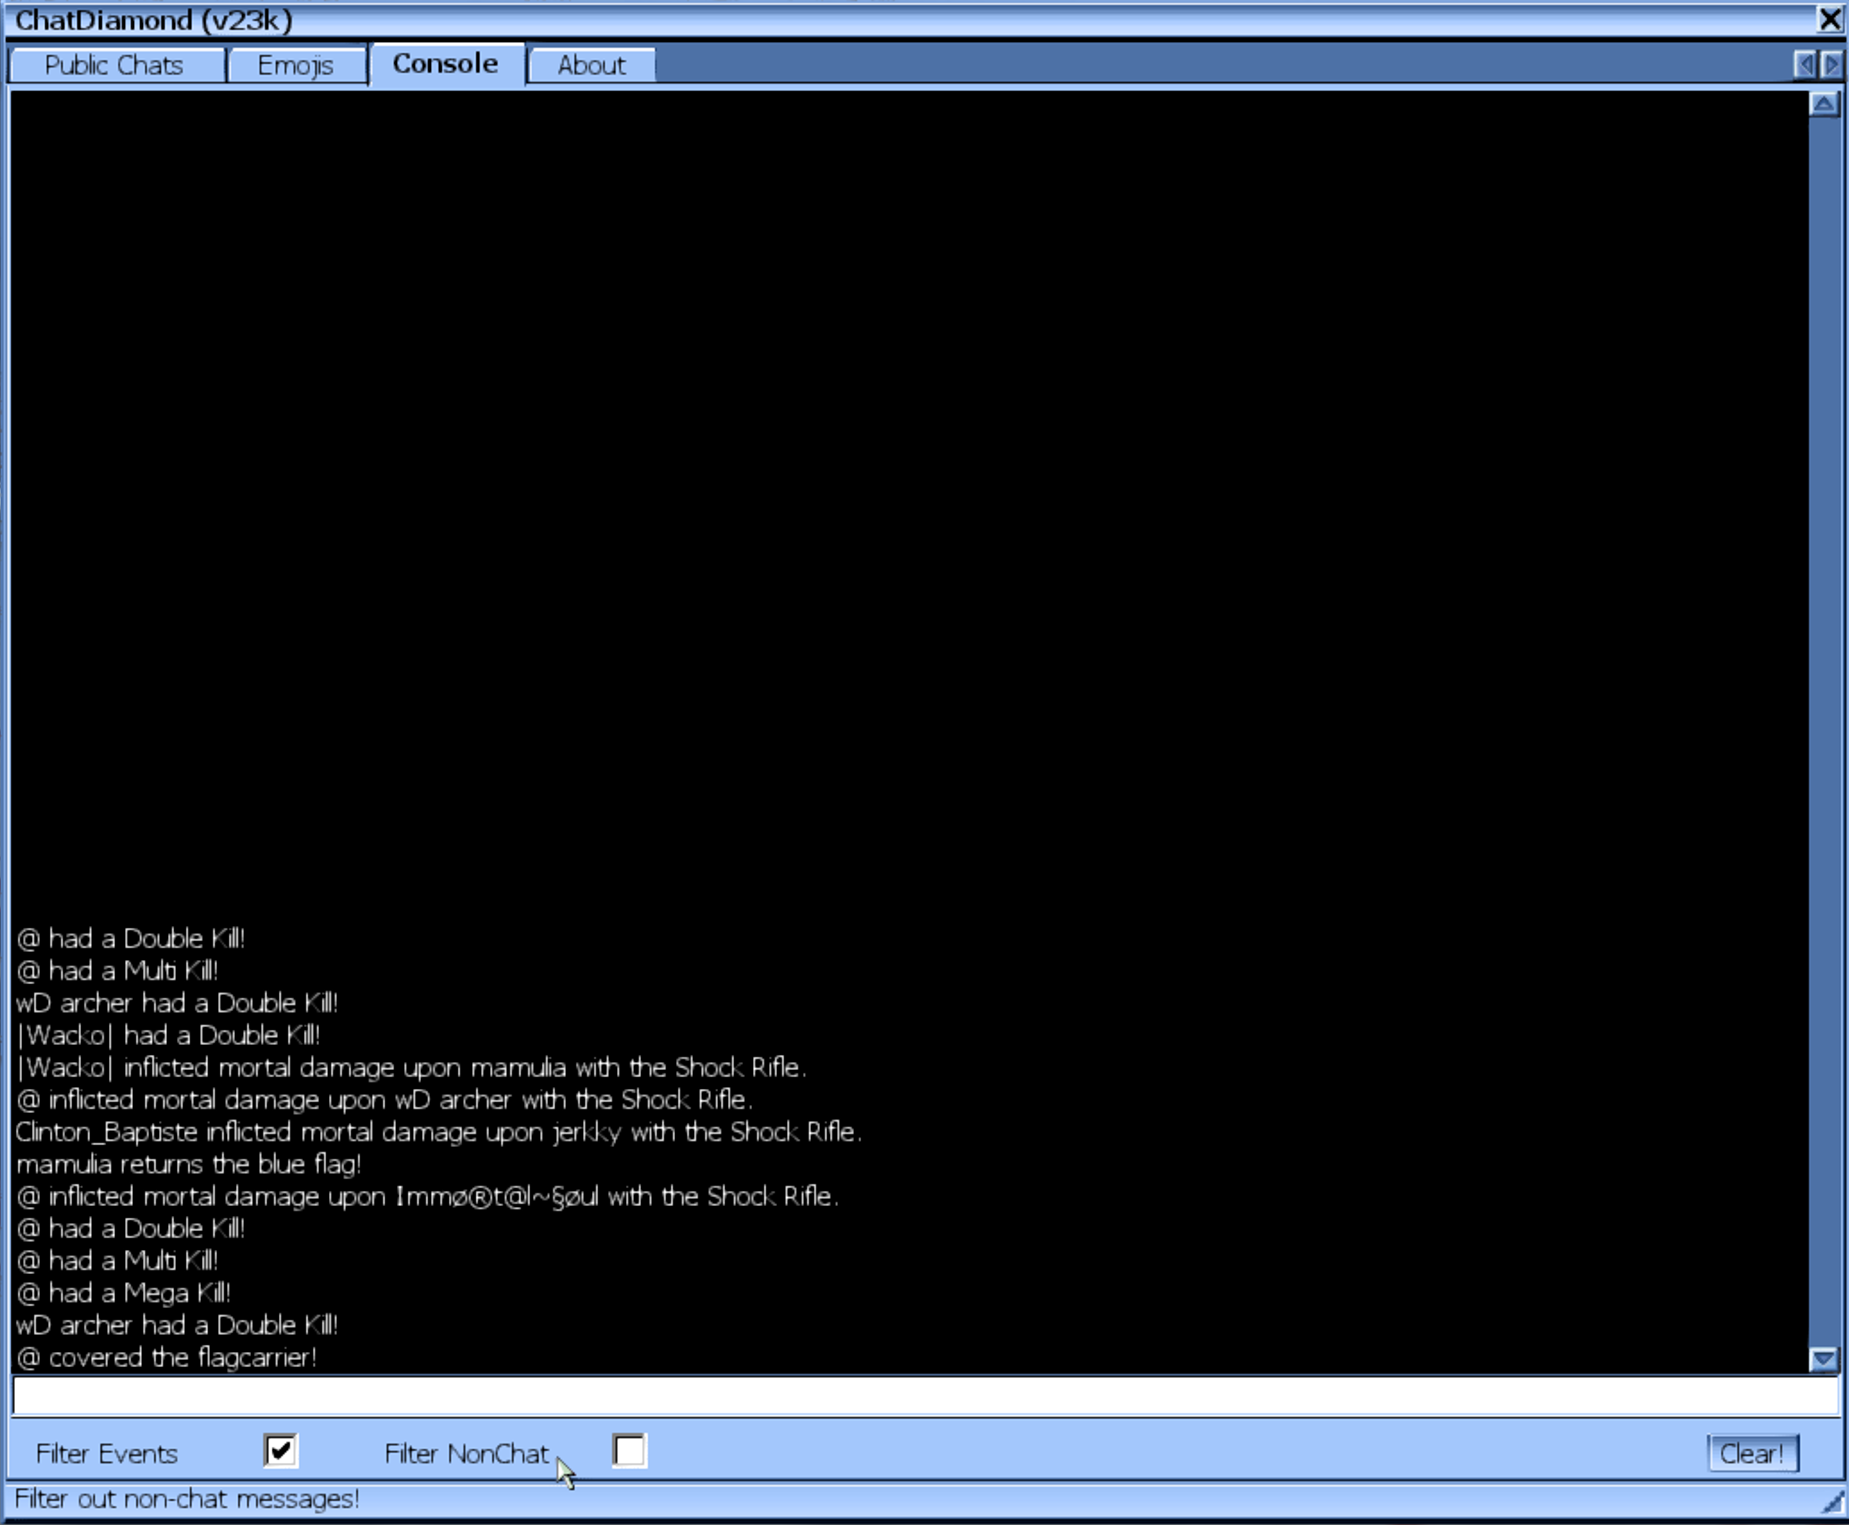
\includegraphics[width=0.4\textwidth]{img_console}
\caption{Chat Diamond \ChatDiamondVersion~Console.}
\label{fig:chatdiamond_console}
\end{figure}

The console now has the following features
\begin{itemize}
\item Non-chat filter to filter out server or mutator advertisements, in the console. Although SmartCTF cover and seal messages may also get filtered.
\item Event filter censors death messages corresponding to the weapon used.
\item A clear button to clean or reset the console.
\item A working status bar linked with console configuration modifiers.
\end{itemize}

\subsection{Configure Window}
Chat Diamond provides ``real time way'' to configure various user configurable parameters.  This implies instant relevant experience on toggling or tuning those parameters, for instance 
tuning the RGB values  for background color of Public Chat window and Console window results in the relevant change in the background of Configure Window itself.   Allow me to provide 
relevant details for configurations
\begin{itemize}
\item \emph{Background Color}: Set the RGB values to come up with a gradation color for backgound.  The setting can be instantaneously applied to Public Chats widow and Console window
\item \emph{Chat Binding}: Click on the box and the key pressed next shall be assigned for opening Public Chats window.
\end{itemize}

\begin{figure}
\centering
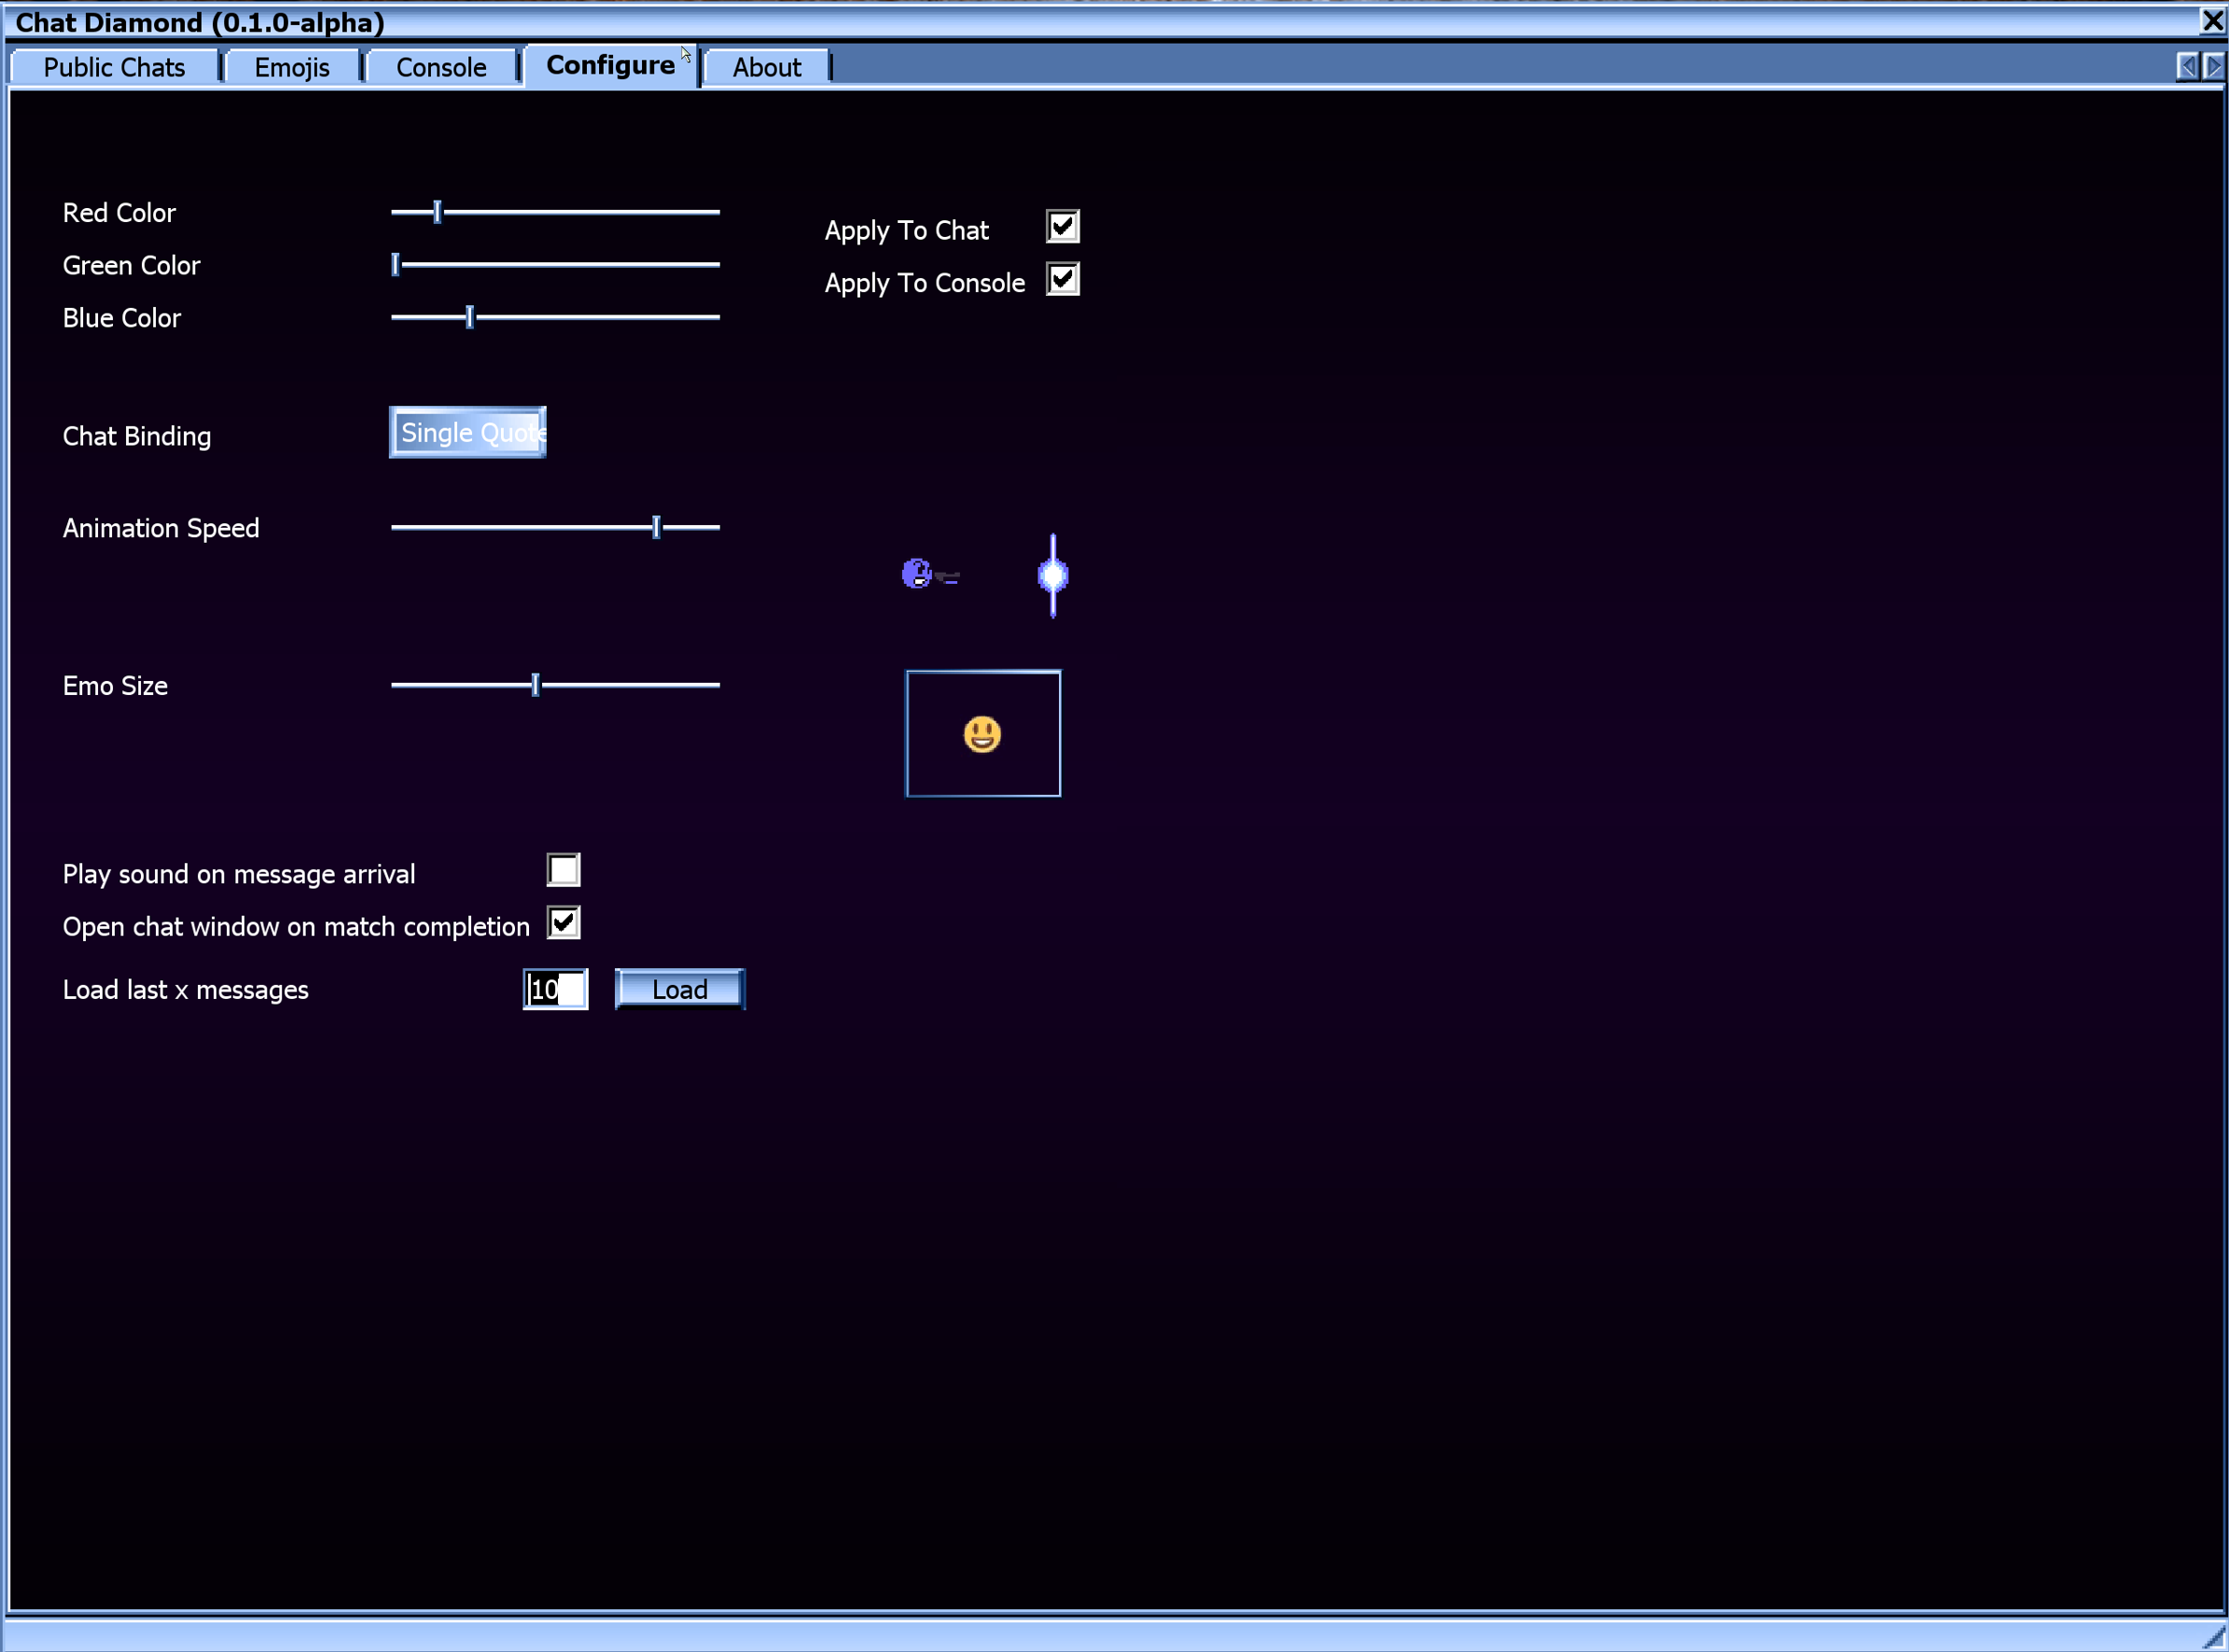
\includegraphics[width=0.4\textwidth]{img_configure}
\caption{Chat Diamond \ChatDiamondVersion~Configure.}
\label{fig:chatdiamond_configure}
\end{figure}


\subsection{More Pages}
Please keep in mind that this is very initial stage of Chat Diamond (\ChatDiamondVersion).  The pages to configure various properties of chat messages
and date format shall be made available as we progress with the development cycle.


\section{Installation}
Chat Diamond is developed and tested with UT99, 469c client.  Although the mod should work on previous versions, I take no pains for maintaining that code simply because I feel that we all should work towards pushing forward the community effort in driving the game (and UE 1) towards modern experience.  So by not supporting the code for earlier versions I am supporting the later versions.

With that being written, feel free to send pull requests to \href{https://github.com/ravimohan1991/ChatDiamond/}{Chat Diamond} repository, even for earlier game versions.

Chat Diamond is essentially a console (and not for the server).  So for installation do the following
\begin{itemize}
\item Place the \FileColor{ChatDiamond.dll} and \FileColor{ChatDiamond.u} files in \FolderColor{System} directory.
\item \FileColor{AkelEditd.lib} is optional file and I'd copy that too in \FolderColor{System} directory just to be safe.
\item Open \FileColor{UnrealTournament.ini} and find the section \\

\fbox{%
    \parbox{\textwidth}{%
       [Engine.Engine]\\
       GameRenderDevice=VulkanDrv.VulkanRenderDevice\\
       AudioDevice=ALAudio.ALAudioSubsystem\\
        \ldots  \\       
       {\color{Green}Console=UTMenu.UTConsole}\\
       \ldots        
    }%
}
\\

\item Modify to \\

\fbox{%
    \parbox{\textwidth}{%
        \ldots  \\       
       {\color{Green}Console=ChatDiamond.CDUTConsole}\\
       \ldots        
    }%
}
\\

\item And that is it!  You can now summon console by usual `$\sim$' key.

\subsection{Configuration}
I am not providing {\color{purple}ChatDiamond.ini}, which should be generated after first successful run of the mod.  
Once that is done make sure to configure the file.  I am in the process of writing the configuration description in full details.

Also embrace for tons of logs about some  ``CDUTChatTextTextureAnimEmoteArea0'' class.  At the moment it skips me on how to suppress the specific logs, if you know you may want to do that and let me know the trick.

I am in the process of resolving the accessed non warnings.

\end{itemize}

\section{Version Histroy}
In this section I am presenting the history of Chat Diamond for general awareness.
\begin{changelog}[author=The\_Cowboy, sectioncmd=\section*]
\begin{version}[v=0.5, date=2023-xx-xx]
  \added
    \item Configure Window
  \fixed
    \item Chat Window text scaling
    \item Emoji Window emojitext offset (\href{https://github.com/ravimohan1991/ChatDiamond/commit/69b7abbce0617ae1c2de0660379984852df9c76d}{69b7abbc})
    \item Chat Window emo textures translucency (\href{https://github.com/ravimohan1991/ChatDiamond/commit/6e105d2cce5db1380c27df546e604d0f306eccd4}{6e105d2c})
    \item Emoji Window emo frames mouse hover detection (\href{https://github.com/ravimohan1991/ChatDiamond/commit/501e585250a6553ca95ca9b9d5e0ad25b1e645b5}{501e5852})
 \changed
    \item Using text file instead of ini for dumping chat metadata (\href{https://github.com/ravimohan1991/ChatDiamond/commit/f059be817532fa720804bd20f54a36e3c82ddb9d}{f059be81})
\end{version}
\shortversion{v=0.1.0-alpha, date=2022-12-25, changes=Initial alpha}
\end{changelog}

\section{A note on UT Messaging}
Chat Diamond's functionality is based upon the tenet ``A complete client side user interface with no dependencies with the server''.  This would imply conforming to the UT standards and any server not conforming to the standards, if so, is not worth visiting.

Based upon the above motivation we have a choice to make between replacing the client HUD or UT console, in order to gather the UT messages client side.  My first instinct was to replace the HUD because that would give more precise classification of the messages, in the sense Epic wrote the code, like \href{http://uncodex.ut-files.com/UT/v436/Source_botpack/challengehud.html}{so} (line 1499)

\begin{lstlisting}[frame=single]
// Entry point for string messages.
simulated function Message( PlayerReplicationInfo PRI, coerce string Msg, name MsgType )
{
    local int i;
    local Class<LocalMessage> MessageClass;

    switch (MsgType)
    {
        case 'Say':
        case 'TeamSay':
            MessageClass = class'SayMessagePlus';
            break;
        case 'CriticalEvent':
            MessageClass = class'CriticalStringPlus';
            LocalizedMessage( MessageClass, 0, None, None, None, Msg );
            return;
        case 'DeathMessage':
            MessageClass = class'RedSayMessagePlus';
            break;
        case 'Pickup':
            PickupTime = Level.TimeSeconds;
        default:
            MessageClass = class'StringMessagePlus';
            break;
     }
   %* \ldots *)           
\end{lstlisting}

The basic premise of many cheats providing aim assist is to modify the HUD client side and display the adversary's position behind the wall or a radar.  This is the reason why modern anti-cheats are not receptive of clients modifying HUD, and thus, work with the concept of ``whitelisting''.

If the notion of ``cheat-anticheat'' interplay exists in the UT standards, then that simply doesn't fit with the tenant we began with.  We don't want to be sending request to server administrators for specifically whitelisting Chat Diamond which will be reverted by cold silent treatment to say the most and some naggy jibber jabber about the unknown-ness of Chat Diamond, especially when the mod is not that popular.

So with this thinking in mind, the better option would be to replace the client console, which I haven't seen any decent anti-cheat prohibiting. This not only gets the client out of hook for sending whitelisting requests but also provides a powerful mechanism to mould the console, specifically for generic needs (see the concept of \emph{filters})\footnote{Althought some servers may prohibit the use of custom consoles.  For that you may have to specifically send the whitelist request. You may want to report the relevant console class, which, for Chat Diamond, should be ``ChatDiamond.CDUTConsole''.}.

\subsection{A minor PhD on console messages}

We start with the \href{http://uncodex.ut-files.com/UT/v436/Source_engine/playerpawn.html}{code} 

\begin{lstlisting}[frame=single]
event ClientMessage( coerce string S, optional Name Type, optional bool bBeep )
{
     %* \ldots *)    
    if (Player.Console != None)
        Player.Console.Message( PlayerReplicationInfo, S, Type );
    if (bBeep && bMessageBeep)
        PlayBeepSound();
    if ( myHUD != None )
        myHUD.Message( PlayerReplicationInfo, S, Type );
}       
\end{lstlisting}
and
\begin{lstlisting}[frame=single]
event TeamMessage( PlayerReplicationInfo PRI, coerce string S, name Type, optional bool bBeep  )
{
    if (Player.Console != None)
        Player.Console.Message ( PRI, S, Type );
    if (bBeep && bMessageBeep)
        PlayBeepSound();
    if ( myHUD != None )
        myHUD.Message( PRI, S, Type );
}     
\end{lstlisting}

It is clear that both the console and HUD should receive same messages with no discrimination (unless if coder specifically demands, as mentioned in \ref{foot:hudconsolediff}).  The console would display them, in what I would like to think, \emph{raw} form.  The \emph{diff}, between console and HUD, is shown in the figure \ref{fig:chatdiamond_console_hud}

\begin{figure}
\centering
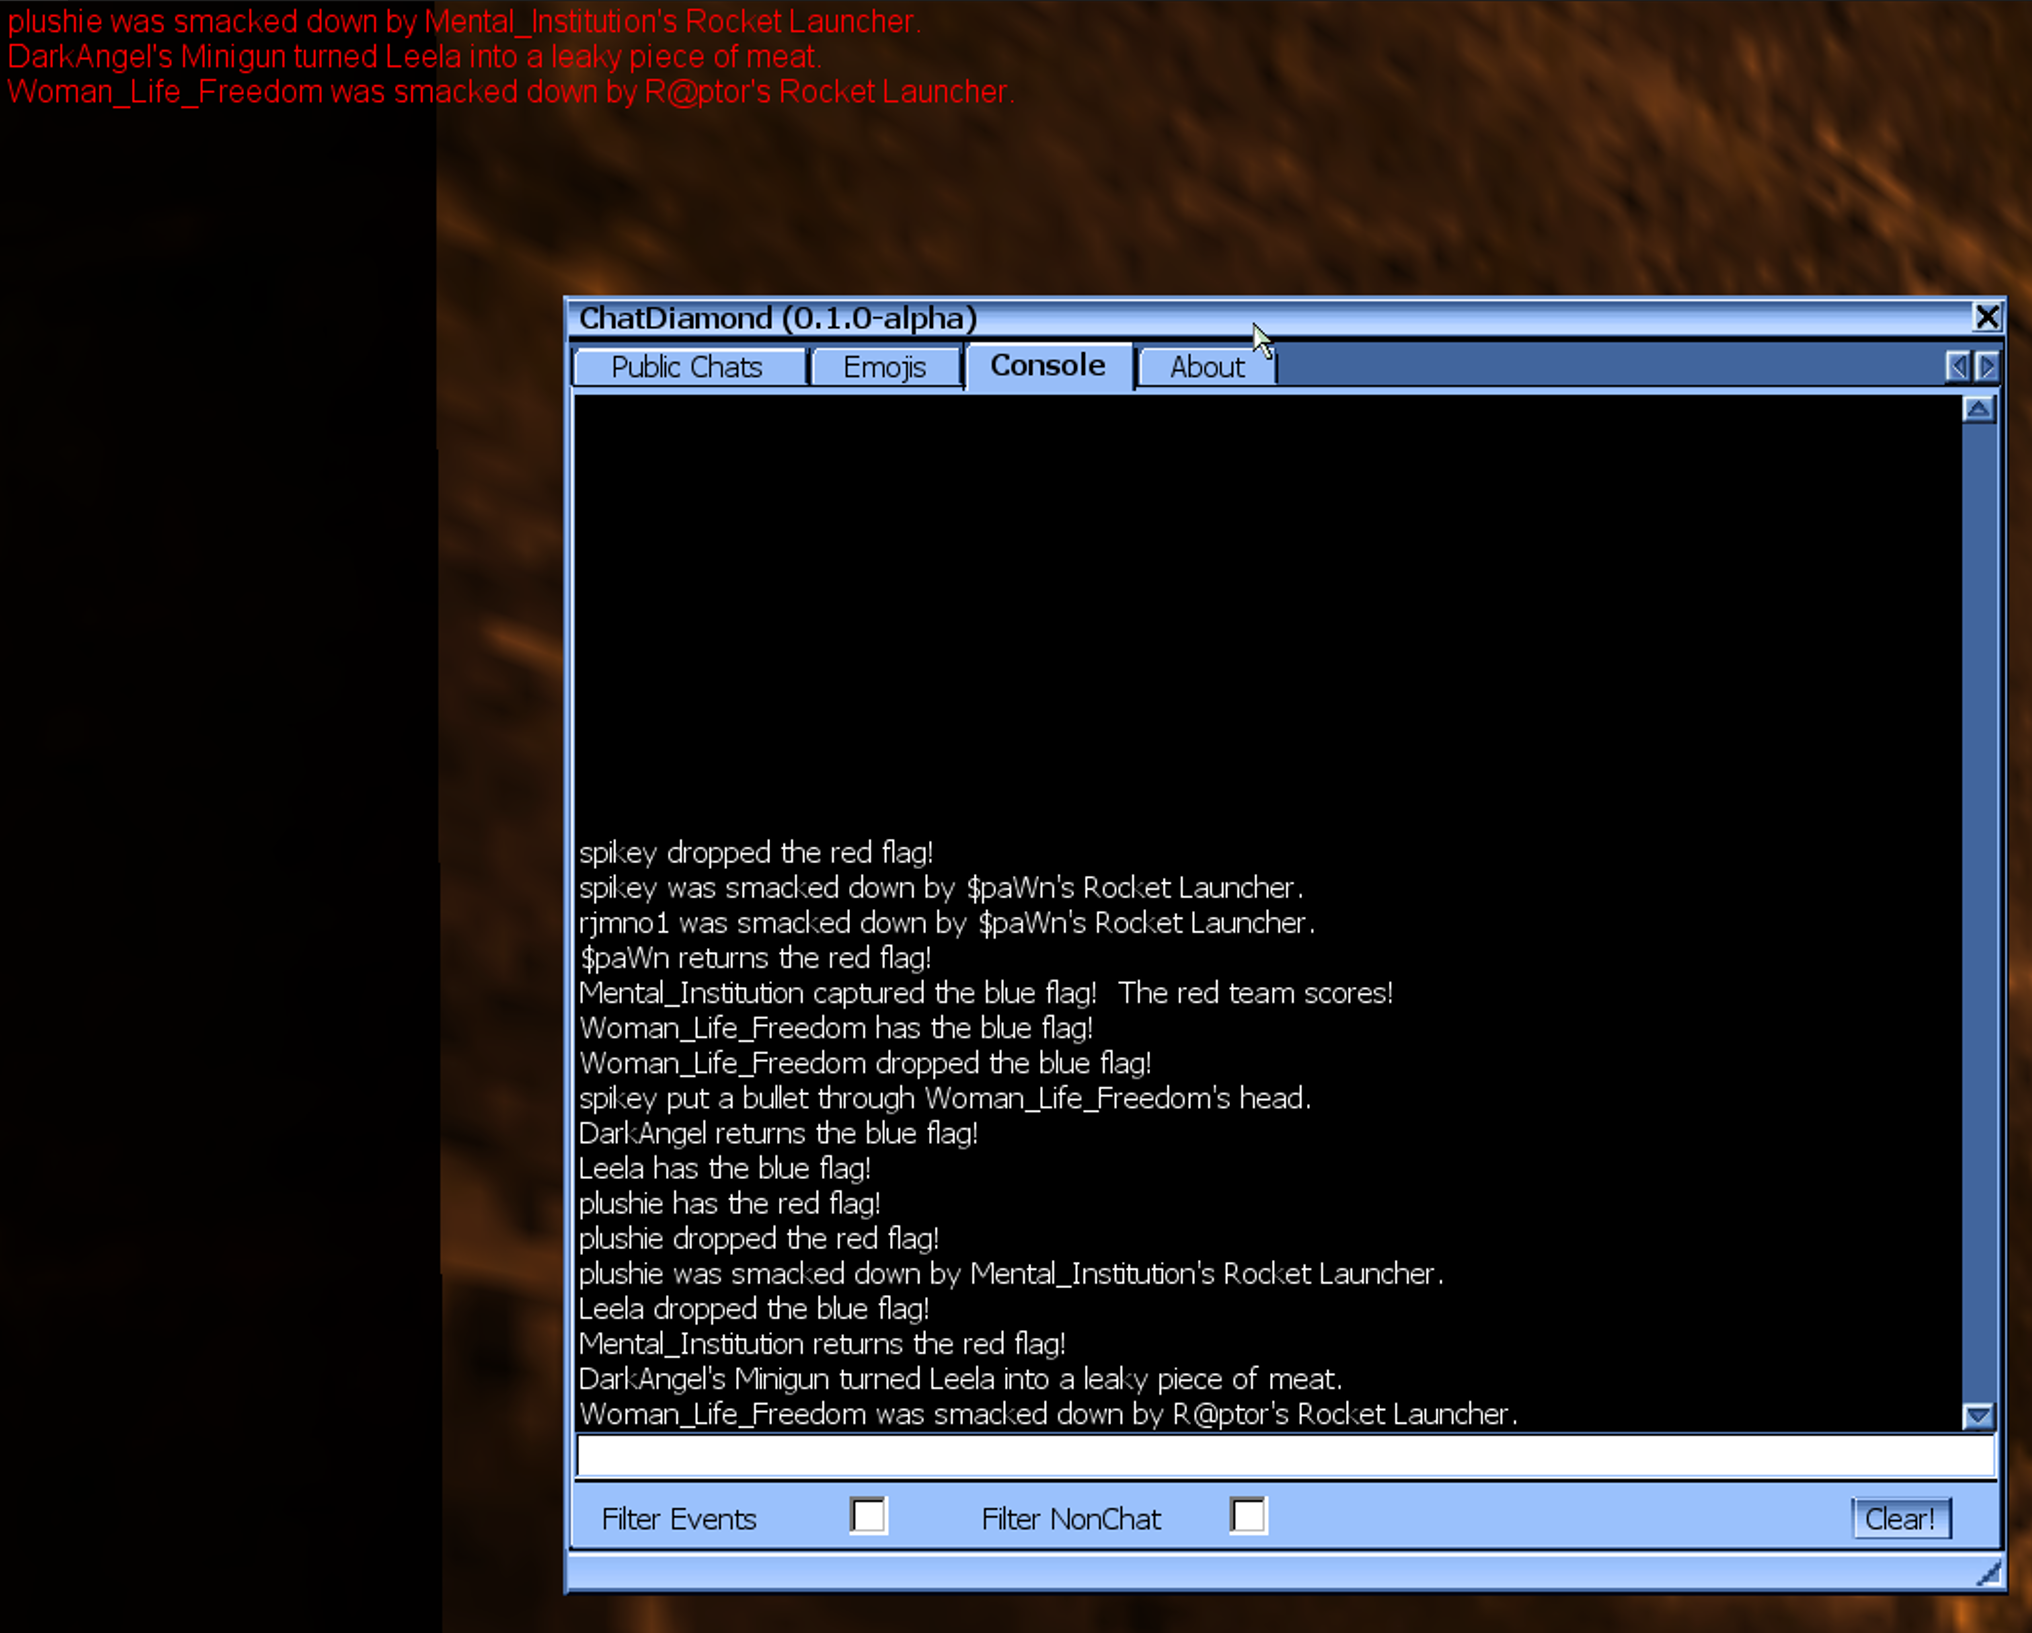
\includegraphics[width=0.4\textwidth]{consoleundhud}
\caption{UT99 HUD with Chat Diamond console}
\label{fig:chatdiamond_console_hud}
\end{figure}

Please note that Chat Diamond's console is not much different from default UT99, visually.  The changes are how Chat Diamond interprets the raw messages thrown and utilize them in a constructive way. So this is where magic \href{https://github.com/ravimohan1991/ChatDiamond/blob/859323fbd80266b21c9dab163b067cacfa318463/Classes/CDUTConsole.uc#L52-L71}{code} comes in.  In order to understand that let me first demonstrate UT messaging by a table\footnote{\label{foot:hudconsolediff} The ``messages'' for instance: `plushie was smacked down by Mental\_Instituitions's Rocket Launcher', are actually strings which can be seen in the line 117 of the \href{http://uncodex.ut-files.com/UT/v436/Source_botpack/deathmessageplus.html}{code}.  This also shows how some death messages can be suppressed in the console thus differing from HUD.}.

The mapping to relevant arguments is like so in Table \ref{tab:messageform}.


The tables need to be explained and pondered.

\section{Native Coding}
Chat Diamond is a native mod, meaning, a program invoking C++ functions.  At the time of writing, minor usage of the library 
\href{https://en.cppreference.com/w/cpp/regex}{regular expressions} is (or should be) evident from the following \href{https://github.com/ravimohan1991/ChatDiamond/blob/6e3b684403fb75811c1cde6372c9125370bc796a/Classes/CDDiscordActor.uc#L61}{code}

\begin{lstlisting}[frame=single]
native final static function string SpitIpFromChatString(string Message, out int ICategory);
\end{lstlisting}

To understand the implementation of the above unreal script function, please see the \href{https://github.com/ravimohan1991/ChatDiamond/blob/6e3b684403fb75811c1cde6372c9125370bc796a/UTNativeEssentials/ChatDiamond/Src/ChatDiamondNative.cpp#L52}{code} displayed as follows

\lstset{language=C++}
\begin{lstlisting}[frame=single]
void ACDDiscordActor::execSpitIpFromChatString(FFrame& Stack, RESULT_DECL)
{
	guard(ACDDiscordActor::execSpitIpFromChatString);
	P_GET_STR(Message);
	P_GET_INT_REF(IPCategory);
	P_FINISH;

	std::smatch Match;

	// The nice way out, from game and web server mix, seems to make an assumption that, in context of UT, the gameserver IP
	// be given by complete port number.

	// https://github.com/ravimohan1991/ChatDiamond/issues/1#issuecomment-1356906185
	std::regex GameIPMould("\\d{1,3}\\.\\d{1,3}\\.\\d{1,3}\\.\\d{1,3}\\:\\d{1,4}");
	std::regex WebIPMould("\\d{1,3}\\.\\d{1,3}\\.\\d{1,3}\\.\\d{1,3}");

	std::wstring WString(*Message);
	std::string SampleString(WString.begin(), WString.end());

	std::string IPString;

	// Look for game IP
	if (std::regex_search(SampleString, Match, GameIPMould))
	{
		for (auto Tempo : Match)
		{
			IPString = Tempo.str();
			break;
		}
	}

	if (!IPString.empty())
	{
		std::wstring WideIPString = std::wstring(IPString.begin(), IPString.end());
		*IPCategory = 0;
		*(FString*)Result = WideIPString.c_str();
		return;
	}

	// Look for game IP
	if (std::regex_search(SampleString, Match, WebIPMould))
	{
		for (auto Tempo : Match)
		{
			IPString = Tempo.str();
			break;
		}
	}

	if (!IPString.empty())
	{
		std::wstring WideIPString = std::wstring(IPString.begin(), IPString.end());
		*IPCategory = 1;
		*(FString*)Result = WideIPString.c_str();
		return;
	}

	std::wstring WideIPString = std::wstring(IPString.begin(), IPString.end());
	*IPCategory = 2;
	*(FString*)Result = WideIPString.c_str();

	unguard;
}
\end{lstlisting}

There are few remarks
\begin{itemize}
\item The C++ code isn't the ordinary one.  That is punctuated with variety of macros, which generate, what I would like to call, the
first hints of reflection system.
\item In order to linearize the story of native coding and start producing practical code, we need to first learn few ``game-dev'' terminologies
and practices.
\end{itemize}

\subsection{Why Native Code?}
Unreal script is a highly managed language which comes with limitations, which is characteristic of any managed language actually, such as slow(er) 
runtime (when compared with C++), ability to fuse with well defined C++ applications (like Discord), and lack of programmers' choice or taste.  Don't get
me wrong, the language is best for what it does, scripting mods for the game.  Since this is 2020 decade, along with native support, there should be no 2000's environment 
limitation, especially with the new community patches.

\subsection{Build System}
I have been using combination of Wot Greal (unrealscript code) and Microsoft Visual Studio 2022 (C++ code) IDEs for developing Chat Diamond.  
Therefore I have organized the repository with the conforming hierarchical structure \ref{forest:project_hierar}.
\begin{figure}
\begin{forest}
  for tree={
    font=\ttfamily,
    grow'=0,
    child anchor=west,
    parent anchor=south,
    anchor=west,
    calign=first,
    edge path={
      \noexpand\path [draw, \forestoption{edge}]
      (!u.south west) +(7.5pt,0) |- node[fill,inner sep=1.25pt] {} (.child anchor)\forestoption{edge label};
    },
    before typesetting nodes={
      if n=1
        {insert before={[,phantom]}}
        {}
    },
    fit=band,
    before computing xy={l=15pt},
  }
[UnrealTournament
  [ChatDiamond (repository)
    [Classes]
    [Sounds]
    [Textures]
    [UTNativeEssentials
        [ChatDiamond
            [Inc(C++)]
            [Src(C++)]
        ]
        [Core]
        [Engine]
        [CamkeLists.txt]
        [GenerateProjectFiles.bat]
    ]
  ]
  [System
    [UnrealTournament.exe]
    [UCC.exe]
  ]
]
\end{forest}
\caption{Chat Diamond project hierarchy.}
\label{forest:project_hierar}
\end{figure}

What we have achieved by doing so is a reconciliation of UT99's unreal script modding environment with C++ dev environment yielding a version controlled  (a Github 
\href{https://github.com/ravimohan1991/ChatDiamond}{repository}) avidity with UT's root folder.  
All the C++ code goes to the folders marked with, well, C++ and unreal script code goes to top level \FolderColor{ChatDiamond \textbackslash Classes} directory.  

The \FolderColor{Core} is the directory containing ``header-only'' library elements, meaning .h files and the already compiled binary \FileColor{Core.lib}.  Few remarks are to be worded
\begin{itemize}
\item Such libraries, which are prebuilt and whose implementation is hidden with only headers (the API) visible, are known as ``\texttt{Interface}'' libraries in CMake's scope.  \FolderColor{Engine} is another example of directory containing such \texttt{Interface} library.  
Also both of the \FolderColor{Engine} and \FolderColor{Core} directories contain the directories \FolderColor{Inc}, \FolderColor{Src}, and \FolderColor{Lib} sub directories. 
\item From research, \FileColor{Core.lib} and \FileColor{Engine.lib}, which are static libraries, seem to be the ``basic necessities'' for linking with a native mod. 
\item In the hierarchy, I am only showing the top level \FileColor{CmakeLists.txt}.  If you are familiar with the build utility, you can comprehend the presence of one each inside \FolderColor{ChatDiamond}, \FolderColor{Core}, and \FolderColor{Engine} directories.
\item Currently, I am developing on and for Windows (should be evident from \FileColor{GenerateProjectFiles.bat}).  It goes against my philosophy of cross-platform development\footnote{For solid enough work please see \href{https://github.com/ravimohan1991/KarmaEngine}{Karma}.} given the 32-bit jugaad for Linux libraries, I may do something in future.  MacOS seems like a workable goal since I own a MacBook Pro.
\end{itemize}  

Make sure that your machine has \href{https://cmake.org/}{CMake} installed.  For uninitiated programmers (in my POV read premakers), let me
supply a crash course on CMake, for our purposes here.

\subsubsection{UT and CMake}
In a C++, or any good programming language, there is a proper tool-chain which pipes the human written code to Turing machine understandable arrangement of bits 
(zeroes and ones).  This usually involves lot of garbage intermediary files which most of the part are useless, unless you suddenly, out of the blue, decide to do 
scavenging some day.

The responsibility of a good build system is to understand such redundancies and provide a manageable way of dealing with chunks of huge memory files.
Let me demonstrate by simple logistics.  

At the time, the Chat Diamond C++ component has about three to four MB worth of code files (.h and .cpp).  
Visual Studio 2022 generates a solution build of about 144 MB worth of memory and the output is \FileColor{ChatDiamond.dll} which is about two MB.  The intermediary files are 
for IDE's (Visual Studio for instance) and compiler (MSVC or Clang) use only and therefore should be dealt separately by a decent build system\footnote{Actually this is the
reinforcement of the concept of Universal Turing Machine.  That a good compiler should be able to generate same set of instructions, i.e. a program, 
which should behave that same way, no matter a laptop or desktop or smart phone.  Please see \href{https://en.wikipedia.org/wiki/Von_Neumann_architecture}{von-Neumann architecture} for a lucid connection 
between Universal Turing Machine concept and PCs or Macbooks.}.

Given the variety of compilers, with even more variety of platforms, CMake is the most suitable build system and friend that a programmer can, well, make and use.  Along with the clear 
distinct folder generation for intermediate files, CMake comes with high degree of configurability, required for build, and compatibility with known compilers\footnote{For a comprehensive list, please visit \href{https://cmake.org/cmake/help/latest/manual/cmake-compile-features.7.html}{here}.}.  
CMake supports the Windows, Unix, and Linux based platforms.

UT99 was officially released and supported on multiple platforms.  The community clearly intends on keeping that flame intact.  Therefore a rocket scientist isn't really needed to gauge the obvious link 
between UT and CMake.

With enough convincing we are now in a position to understand the organization of this project (or some UT project organization, in general).  This may serve as a template.  
Consider the hierarchy \ref{forest:project_hierar}.  Then the \href{https://github.com/ravimohan1991/ChatDiamond/blob/f7950b2591b93a54600459ec58d7ddf57fe9218d/UTNativeEssentials/CMakeLists.txt#L201-L216}{code}

\lstset{language=[5.0]Lua}
\begin{dummy}
\begin{lstlisting}[frame=single]
###################
# Link Directories
###################
link_directories(ChatDiamond Core/Lib Engine/Lib)

###########################################
# Target Definitions / Custom Modding Stuff
###########################################
add_subdirectory(ChatDiamond)
target_include_directories(ChatDiamond
    PRIVATE
    ${CMAKE_CURRENT_SOURCE_DIR}/Core/Inc
    ${CMAKE_CURRENT_SOURCE_DIR}/Engine/Inc)


######################
# Target Linking Rules
######################
target_link_libraries(ChatDiamond PUBLIC Core Engine)
\end{lstlisting}
\end{dummy}
becomes relevant as follows.

In line 4, we are telling CMake to generate relevant project files (for MSVC or QTCreator) such that the linking can be done with the libraries stored in the \FolderColor{Core\textbackslash Lib} and \FolderColor{Engine\textbackslash Lib} directories\footnote{Note that directories are relative to the current CMake operation directory which is basically the location of the \FileColor{CMakeLists.txt} with above code.}.

Next from line 9 to 13, we intend to tell CMake to add the native mod project, specified by \FileColor{CMakeLists.txt} present in sub-directory \FolderColor{ChatDiamond}.

Next we proceed towards the file mentioned in previous paragraph (taking a level deep plunge in the folder hierarchy).  The \href{https://github.com/ravimohan1991/ChatDiamond/blob/f7950b2591b93a54600459ec58d7ddf57fe9218d/UTNativeEssentials/ChatDiamond/CMakeLists.txt}{code} is
\lstset{language=[5.0]Lua}
\begin{lstlisting}[frame=single]
cmake_minimum_required(VERSION 3.0.0)

project(ChatDiamond)

file(GLOB CD_HEADERS Inc/*.h)

add_library(ChatDiamond SHARED Src/ChatDiamondNative.cpp ${CD_HEADERS})

target_include_directories(ChatDiamond
    PRIVATE
        ${CMAKE_CURRENT_SOURCE_DIR}/Inc
    PUBLIC
        $<BUILD_INTERFACE:${CMAKE_CURRENT_SOURCE_DIR}/Inc>
        $<INSTALL_INTERFACE:${CMAKE_INSTALL_INCLUDEDIR}>
)

target_compile_definitions(ChatDiamond PUBLIC ChatDiamond)
\end{lstlisting}

Line 3 declares the mod project name.  Then we specify all the .h files by collectively assembling them with the command \texttt{file} and labeling them \emph{CD\_HEADERS}.  Then we specify the library name via \texttt{add\_library} command in the first field, followed by the type (\texttt{SHARED} means dynamic library) followed by all the source (.cpp) files.  Then we mention headers so that they may appear nicely in the project.  For instance, in XCode the project ChatDiamond looks like
\begin{figure}
\centering
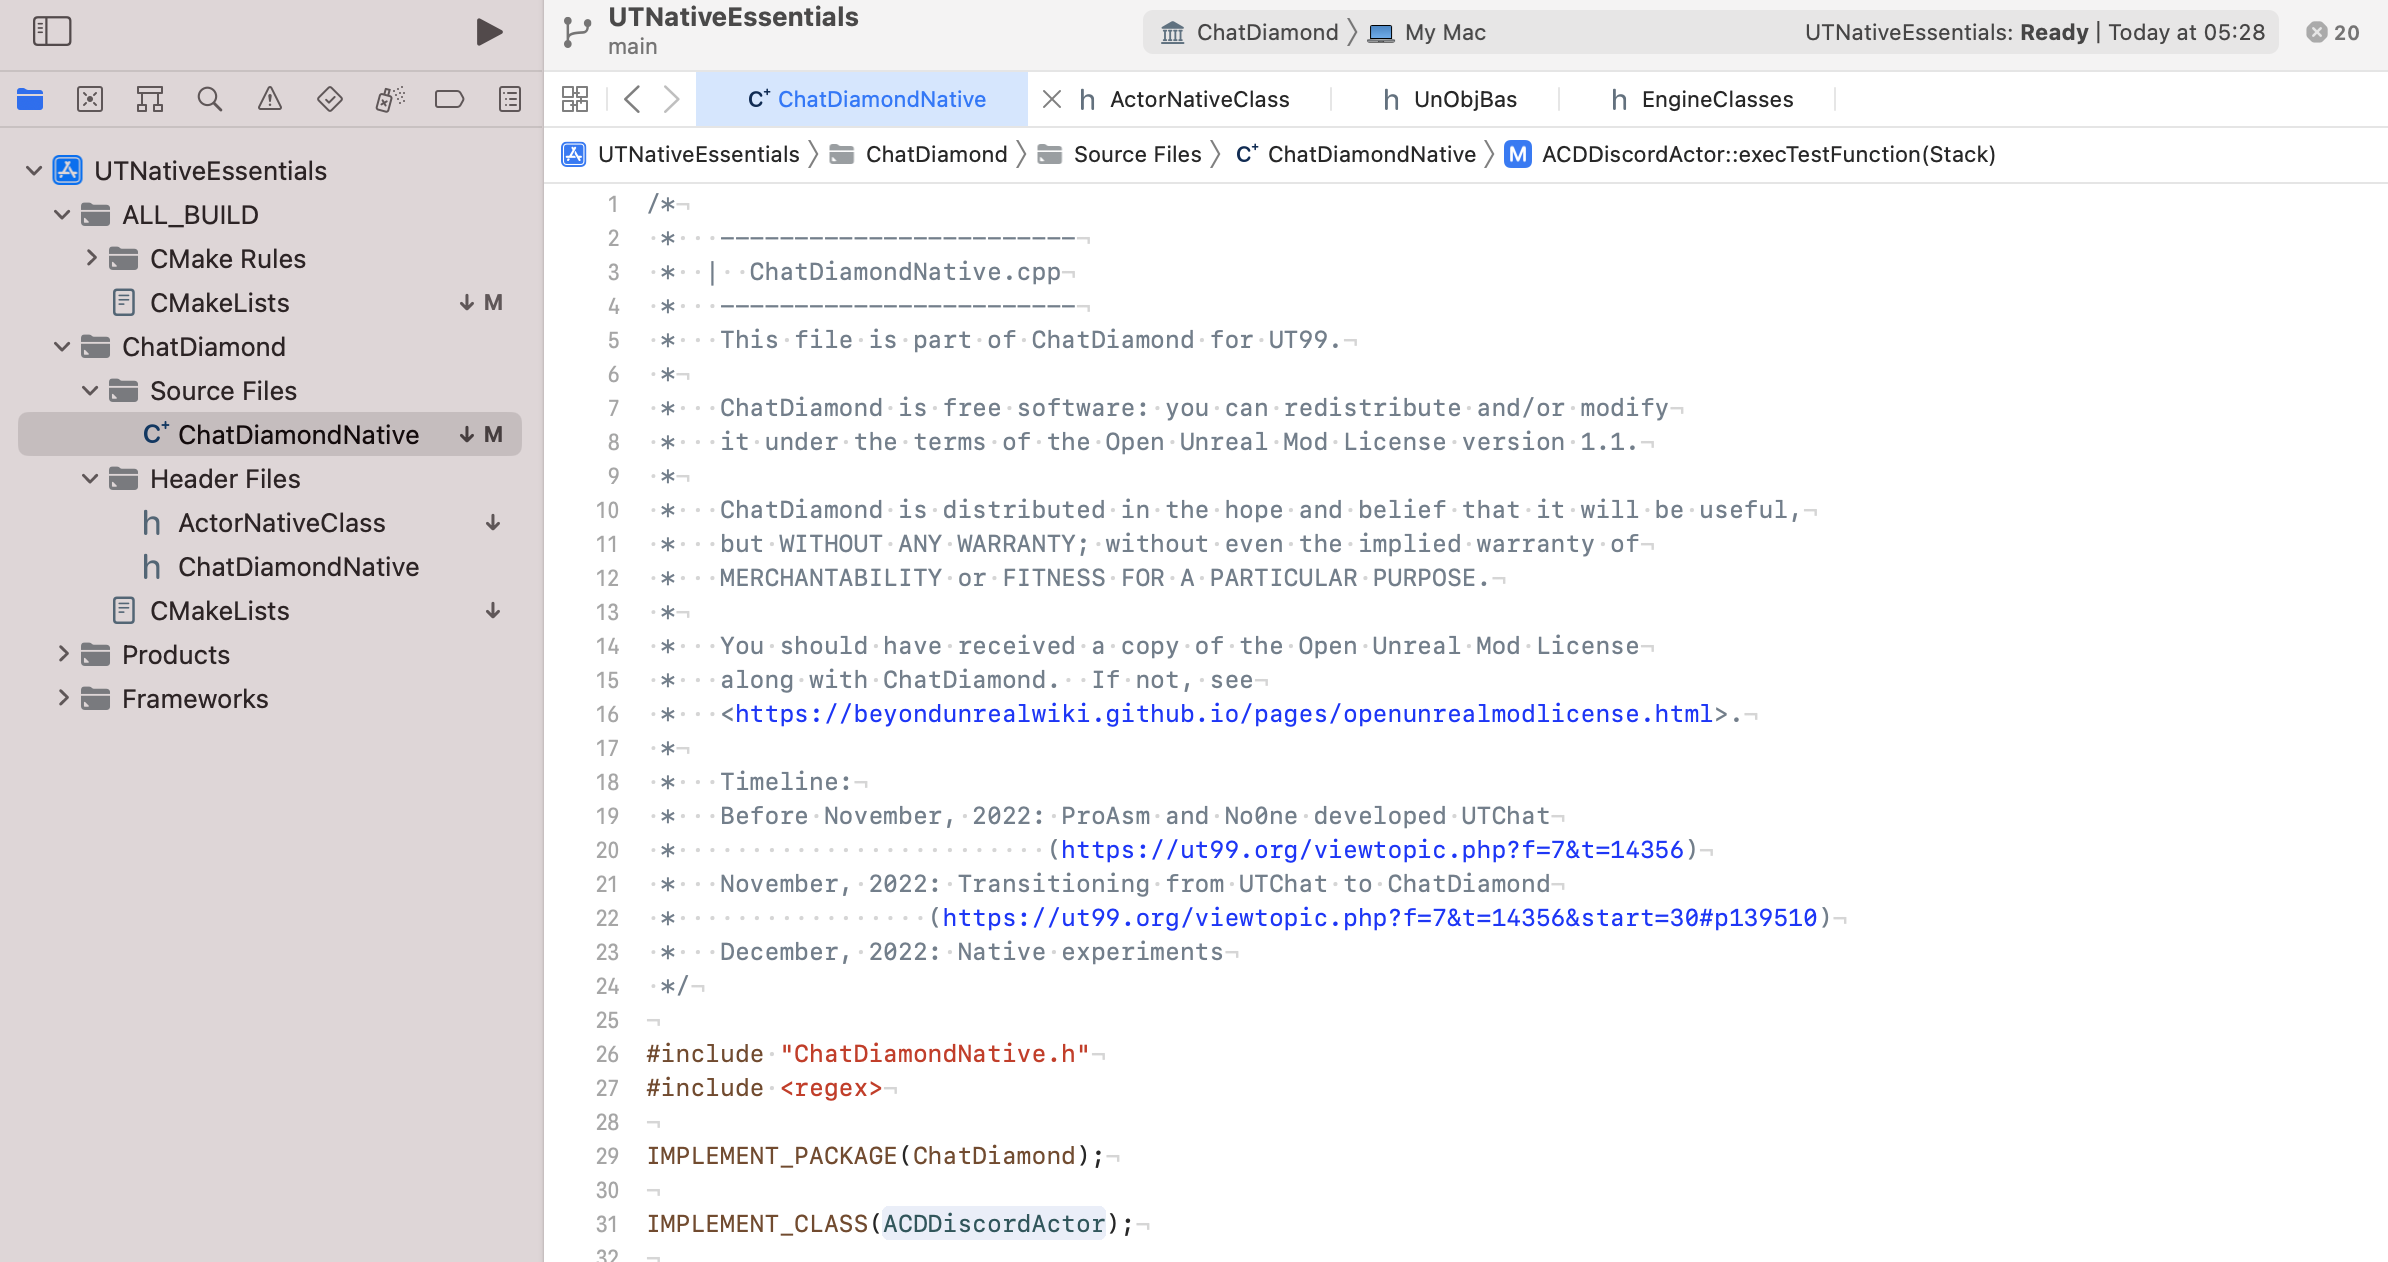
\includegraphics[width=0.9\textwidth]{chatdiamond_xcode}
\caption{A Chat Diamond XCode project.}
\label{fig:chatdiamond_xcode}
\end{figure}

Furthermore we apprise the CMake that the target, ChatDiamond library, needs the includes of \FolderColor{Inc} and provides the same folder as API for various libraries to utilize the functionality.  Finally we set the public usable name, which is same, of the library.

Now we come back to the topmost \FileColor{CMakeLists.txt}, line 10, which can be regarded the continuation of \texttt{target\_include\_directories} of the previous one.  Here we want to tell CMake to include the library directories (the basic essentials) \FolderColor{Core\textbackslash Inc} and \FolderColor{Engine\textbackslash Inc} in our ChatDiamond project and in line 19 we apprise CMake to link those libraries thus generating the wholesome \FileColor{ChatDiamond.dll}, if we are on Windows\footnote{On Linux based OS, the dynamic library has the extension of ``.so'', which stands for ``shared object''.}.

\subsection{C++ for UT}
We are basically in the territory of interface between unreal script and C++ for the game UT99.  Remember the C++ standard that the UT99 was written in could have been C98 (or SO/IEC 14882:1998) and unreal script could have had influences.

In 2022, we can be using any standard ranging from C++11 to C++20.  In CMake above, we defined the standard like \href{https://github.com/ravimohan1991/ChatDiamond/blob/f7950b2591b93a54600459ec58d7ddf57fe9218d/UTNativeEssentials/CMakeLists.txt#L11}{so}

\lstset{language=[5.0]Lua}
\begin{lstlisting}[frame=single]
set(CMAKE_CXX_STANDARD 11)
\end{lstlisting}

This is what we mean by ``modern'', the ability to take good parts from the standards in history of C++ evolution.  With this modern approach, we can leverage the latest  XCode or Microsoft's Visual Studio features (including smarter intellisense) and produce the code that can and will work in future. 

First a shout out to fellas at OldUnreal (and the \href{https://www.oldunreal.com/phpBB3/viewtopic.php?f=37&t=3938}{thread}) for the native ``Hello World'' tutorial and Anthrax for \href{https://github.com/stijn-volckaert/udemo}{UDemo}, a working native mod with useful UT oriented C++ information.

With credits out of the way, let me focus upon the juice.  The aim is to write a C++ function which can be called from unreal script  and which can print

\lstset{language=[5.0]Lua}
\begin{lstlisting}[frame=single]
Log: Hello World! S=Test,I=888
\end{lstlisting}

in the logs.  The idea is to compile a uscript\footnote{I am using unreal script and uscript interchangeably in this document.} code (.u package) which makes the call to native function 
declared within uscript like \href{https://github.com/ravimohan1991/ChatDiamond/blob/f7950b2591b93a54600459ec58d7ddf57fe9218d/Classes/CDDiscordActor.uc#L43}{so}

\lstset{language=Java}
\begin{lstlisting}[frame=single]
native final function bool TestFunction(string S, int I);
\end{lstlisting}

written in \FileColor{CDDiscordActor.uc}.  We need to define this routine in C++, the language the Engine is written in.  That requires punctuation of .h/.cpp files with lot of macros dedicated towards
making Engine understand and adapt to uscript capabilities (modularity, swift iteration, and prototyping functionality\footnote{You can literally use notepad for uscripts if you know what you are doing.}).

We start with the following \href{https://github.com/ravimohan1991/ChatDiamond/blob/f7950b2591b93a54600459ec58d7ddf57fe9218d/UTNativeEssentials/ChatDiamond/Inc/ActorNativeClass.h}{code} analysis
\lstset{language=C++}
\begin{lstlisting}[frame=single]
#if ((_MSC_VER) || (HAVE_PRAGMA_PACK))
#pragma pack (push,4)
#endif

#ifndef NAMES_ONLY
#define AUTOGENERATE_FUNCTION(cls,idx,name)
#endif
\end{lstlisting}

Line 1 is preprocessor instruction which says that if I am using MSVC compiler and if \texttt{HAVE\_PRAGMA\_PACK} is set then the alignment of the aggregate members\footnote{For revisiting the notion of 
members, please see APPENDIX \ref{sec:aggregation}} is defined like \href{https://www.ibm.com/docs/en/zos/2.1.0?topic=descriptions-pragma-pack}{so}

\begin{definition}
Align structure or class members on 4-byte boundaries, or on their natural alignment (see APPENDIX \ref{append:pragma_pack}) boundary\footnote{}, whichever is less.
\end{definition}

\texttt{push} is used to make the alignment contextual.  Therefore you shall find the closing counterpart like \href{https://github.com/ravimohan1991/ChatDiamond/blob/f7950b2591b93a54600459ec58d7ddf57fe9218d/UTNativeEssentials/ChatDiamond/Inc/ActorNativeClass.h#L62}{so}

\lstset{language=C++}
\begin{lstlisting}[frame=single]
#if ((_MSC_VER) || (HAVE_PRAGMA_PACK))
#pragma pack (pop)
#endif
\end{lstlisting}

Thanks to stackoverflow \href{https://stackoverflow.com/questions/3318410/pragma-pack-effect}{discussion}.  I don't quite yet know the relevance to uscript, all I can think is maybe this is UT99's convention 
of dealing with the electronics of 1999 or something.  Also anth (2022) has justification like \href{https://github.com/ravimohan1991/ChatDiamond/blob/f7950b2591b93a54600459ec58d7ddf57fe9218d/UTNativeEssentials/Core/Inc/UnBuild.h#L154-L155}{so}.

Lines 5 to 7 are the instructions that seem redundant for our purposes because we haven't used or don't need the macro for printing the log in my foreseeable way.

Now we come to the actual definition of the class.  As per UT's naming convention all actor names start with `A'.  Hence we have

\lstset{language=C++}
\begin{lstlisting}[frame=single]
class ACDDiscordActor : public AActor
{
public:
	DECLARE_FUNCTION(execTestFunction)
	DECLARE_CLASS(ACDDiscordActor, AActor, 0, ChatDiamond);
	ACDDiscordActor();
};
\end{lstlisting}

Here we need to first understand the \texttt{DECLARE\_FUNCTION} and \texttt{DECLARE\_CLASS} macros.  For the former the definition is like \href{https://github.com/ravimohan1991/ChatDiamond/blob/5592fef2b13305e441c1dd2b09dde7dd52ff2d83/UTNativeEssentials/Core/Inc/UnObjBas.h#L829}{so}

\lstset{language=C++}
\begin{lstlisting}[frame=single]
#define DECLARE_FUNCTION(func) void func( FFrame& TheStack, RESULT_DECL );
\end{lstlisting}

where \texttt{FFrame} is the data structure defined like \href{https://github.com/ravimohan1991/ChatDiamond/blob/5592fef2b13305e441c1dd2b09dde7dd52ff2d83/UTNativeEssentials/Core/Inc/UnStack.h#L273}{so}.  Anth already has full fledged explanation about the inner working and this is how
the train of C++ logic runs

\begin{itemize}
\item The \texttt{UObject::ProcessEvent} is the entry point for unrealscript code, see the \texttt{UFUnction} \href{https://github.com/ravimohan1991/ChatDiamond/blob/5592fef2b13305e441c1dd2b09dde7dd52ff2d83/UTNativeEssentials/Core/Inc/UnClass.h#L379}{code} for instance, where the C++ routine sets a top-level 
\texttt{FFrame}.  Of course, the implementation of \texttt{ProcessEvent} is hidden as of now.
\item The \texttt{ProcessEvent} then sets up stack for uscript function parameters and local variables.
\item The function parameters are then initialized by copying values from \texttt{void* Params} buffer to the top level
 \texttt{FFrame}.
\item  We then execute opcodes one by one using this top-level FFrame as our uscript execution stack until we reach an \texttt{EX\_Return}
opcode or until we hit the end of the function.
\end{itemize}

Note: I don't know what opcode is.

\texttt{DECLARE\_CLASS} is defined like \href{https://github.com/ravimohan1991/ChatDiamond/blob/5592fef2b13305e441c1dd2b09dde7dd52ff2d83/UTNativeEssentials/Core/Inc/UnObjBas.h#L421}{so}

\lstset{language=C++}
\begin{lstlisting}[frame=single]
// Declare a concrete class.
#define DECLARE_CLASS( TClass, TSuperClass, TStaticFlags, ... ) \
	DECLARE_BASE_CLASS( TClass, TSuperClass, TStaticFlags, __VA_ARGS__ ) \
	friend FArchive &operator<<( FArchive& Ar, TClass*& Res ) \
		{ return Ar << *(UObject**)&Res; } \
	virtual ~TClass() noexcept(false)   \
		{ ConditionalDestroy(); } \
	static void InternalConstructor( void* X ) \
		{ new( (EInternal*)X )TClass; } \
\end{lstlisting}

where \texttt{DECLARE\_BASE\_CLASS} is defined like \href{https://github.com/ravimohan1991/ChatDiamond/blob/5592fef2b13305e441c1dd2b09dde7dd52ff2d83/UTNativeEssentials/Core/Inc/UnObjBas.h#L380}{so}

\lstset{language=C++}
\begin{lstlisting}[frame=single]
#define DECLARE_BASE_CLASS( TClass, TSuperClass, TStaticFlags, ... ) \
public: \
	/* Identification */ \
	enum {StaticClassFlags=TStaticFlags}; \
	private: static UClass PrivateStaticClass; public: \
	typedef TSuperClass Super;\
	typedef TClass ThisClass;\
	static UClass* StaticClass() \
		{ return &PrivateStaticClass; } \
	void* operator new( size_t Size, UObject* Outer=(UObject*)GetTransientPackage(), FName Name=NAME_None, DWORD SetFlags=0 ) \
		{ return StaticAllocateObject( StaticClass(), Outer, Name, SetFlags ); } \
	void* operator new( size_t Size, EInternal* Mem ) \
		{ return (void*)Mem; }
\end{lstlisting}

So, on macro expansion, the code takes the following nice lucid form

\lstset{language=C++}
\begin{lstlisting}[frame=single]
class ACDDiscordActor : public AActor
{
public:
	ACDDiscordActor();

public:
	void execTestFunction(FFrame& TheStack, void* const Result);

public:
public: 
	/* Identification */
	enum { StaticClassFlags = 0 };
	private: static UClass PrivateStaticClass; 

public:
	typedef AActor Super;
	typedef ACDDiscordActor ThisClass;
	static UClass* StaticClass()
	{
		return &PrivateStaticClass; 
	}
	void* operator new(size_t Size, UObject* Outer = (UObject*)GetTransientPackage(), FName Name = NAME_None, DWORD SetFlags = 0)
	{
		return StaticAllocateObject(StaticClass(), Outer, Name, SetFlags); 
	}
	void* operator new(size_t Size, EInternal* Mem)
	{
		return (void*)Mem;
	}

	friend FArchive& operator<<(FArchive& Ar, ACDDiscordActor*& Res)
	{ 
		return Ar << *(UObject**)&Res; 
	}
	virtual ~ACDDiscordActor() noexcept(false)
	{
		ConditionalDestroy(); 
	}
	static void InternalConstructor(void* X)
	{
		new((EInternal*)X)ACDDiscordActor;
	}
};
\end{lstlisting}

Now we come to the definition of the function done like \href{https://github.com/ravimohan1991/ChatDiamond/blob/5592fef2b13305e441c1dd2b09dde7dd52ff2d83/UTNativeEssentials/ChatDiamond/Src/ChatDiamondNative.cpp#L43}{so}

\lstset{language=C++}
\begin{lstlisting}[frame=single]
void ACDDiscordActor::execTestFunction(FFrame& Stack, RESULT_DECL)
{
	guard(ACDDiscordActor::execTestFunction);
	P_GET_STR(S);//Get the first parameter
	P_GET_INT(I);//and the second
	P_FINISH;//you MUST call this or it will crash.

	GLog->Logf(TEXT("Hello World! S=%s,I=%i"), *S, I);//Log output and use printf format.
	//You may also use debugf(TEXT("Hello world!")) since it may be easier to remember.
	*(UBOOL*)Result = true;// Return true to UScript, this is how you return a result. You cast your result into "Result" -- whatever it may be.
	unguard;
}
IMPLEMENT_FUNCTION(ACDDiscordActor, -1, execTestFunction);
\end{lstlisting}

Most parts have been explained in comments.  I shall focus on the following

\begin{itemize}
\item \texttt{P\_GET\_STR} is defined like \href{https://github.com/ravimohan1991/ChatDiamond/blob/5592fef2b13305e441c1dd2b09dde7dd52ff2d83/UTNativeEssentials/Core/Inc/UnScript.h#L63}{so}
\lstset{language=C++}
\begin{lstlisting}[frame=single]
#define P_GET_STR(var)                FString var;                         Stack.Step( Stack.Object, &var    );
#define P_GET_INT(var)                INT   var=0;                         Stack.Step( Stack.Object, &var    );
\end{lstlisting}
is used for collecting the arguments of our uscript function \texttt{TestFunction(string S, int I)} and order is indespensible.
\item \texttt{P\_FINISH} is defined like so

\lstset{language=C++}
\begin{lstlisting}[frame=single]
#define P_FINISH                      Stack.Code++;
\end{lstlisting}

\end{itemize}

\appendix

\section{Messaging Tables}

\begin{tabcontainer}
 \begin{tabularx}{\textwidth}{| X | X | X | X |}
 \hline
 \makecell{Console\\ Owner\\ State} & \makecell{Death\\ Messages}\footnote{A string rather.  See \ref{foot:hudconsolediff}}  & \makecell{Server\\ Announcements\footnote{Server adds?}} & \makecell{Talk \\ TeamTalk} \\ [0.5ex] 
 \hline\hline
 
\makecell{Multiplayer \\Spectator} & \makecell{\color{red}{plushie was}\\ \color{red}{smacked down}\\ \color{red}{by MI's}\\ \color{red}{Rocket Launcher}} & \makecell{Type !cg to\\ visit combogib\\ grapple server}  & \makecell{A: Self Sent- \\RN\footnote{Receiver's (who is spectator) Name}:Hola\\  \\ B. By Player-\\ RN:SN\footnote{Sender's name, who is a player.}:Hola \\ \\ C. By spectator\footnote{A different spectator}\\ SN:Hola}\\

\hline
  \end{tabularx}
  \caption{Table of Messages.}
  \label{tab:messform}
\end{tabcontainer}

\begin{tabcontainer}
 \begin{tabularx}{\textwidth}{| X | X | X | X |}
 \hline
 \makecell{Console\\ Owner\\ State} & \makecell{Death\\ Messages}\footnote{A string rather.  See \ref{foot:hudconsolediff}}  & \makecell{Server\\ Announcements\footnote{Server adds?}} & \makecell{Talk \\ TeamTalk} \\ [0.5ex] 
 \hline\hline
 
\makecell{Multiplayer \\Spectator} & \makecell{MessageType:  \\ DeathMessage?\\ \\ PRI:  Local?} & \makecell{MessageType:\\ Event \\  \\ PRI: Local}  & \makecell{A. \\ MessageType:\\ Event  \\ PRI: Local \\ \\  B.\\ MessageType: \\ Event \\ PRI: local\\ \\ C. \\  MessageType: \\ Event \\ PRI: Local}\\
    \hline

\makecell{Multiplayer\\ Player} & \makecell{Message Type: \\ Event \\ PRI: Local? } & \makecell{Message Type: \\ Event \\ PRI: None} & \makecell{A. \\ MessageType: \\ Say\\ PRI: Local\\ \\ B. \\ MessageType: \\ Say \\ PRI: SenderPRI \\ \\ C. \\ MessageType: \\ ? \\ PRI: ?}\\
    \hline
  \end{tabularx}
  \caption{Table of argument types.}
  \label{tab:messageform}
\end{tabcontainer}

\section{Aggregation}
\label{sec:aggregation}
In C++, aggregation is a process in which one class defines another class as any entity reference. It is another way to reuse the class. It is a form of association that represents HAS-A relationship.

\lstset{language=C++, framexleftmargin=5mm, frame=shadowbox, rulesepcolor=\color{blue}}
\begin{dummy}
\begin{lstlisting}[frame=single]
class Address
{  
    public:
    string addressLine;
    Address(string addressLine)
    {    
        this->addressLine = addressLine;
    }
};
class Employee
{
    private:
    Address* address;  //Employee HAS-A Address

    public:
    int id;
    Employee(int id, Address* address)
    {
        this->id = id;
        this->address = address;
    }
    void display()
    {
        cout<<id <<"\n";
        address->addressLine;
    }
};
\end{lstlisting}
\end{dummy}
In the code above, line 13 is the example of aggregate member \texttt{address}.

\section{\#pragma pack}
\label{append:pragma_pack}
First a definition

\begin{definition}
Natural alignment roughly means data's memory address is multiple of data size.
\end{definition}

For instance, in a 32-bit architecture, the data may be aligned if the data is stored in four consecutive bytes and the first byte lies on a 4-byte boundary.  
Thus if there is a class like so

\lstset{language=C++, framexleftmargin=5mm, frame=shadowbox, rulesepcolor=\color{blue}}
\begin{lstlisting}[frame=single]
class Test
{
    char a;
    int b;
};
\end{lstlisting}

then, if natural alignment is done (say 32 bit, or x86, architecture), the size of \texttt{Test} would be 8 bytes with the following breakdown
\begin{itemize}
\item 1 char byte + 3 bytes of padding
\item 4 bytes for int
\end{itemize}

\end{document}